\documentclass{article}
\usepackage{neurips_2026}
% neurips_2026 already loads: natbib
\usepackage{amsthm}
\usepackage{bbm}
\usepackage{amssymb}
\usepackage[utf8]{inputenc} % allow utf-8 input
\usepackage[T1]{fontenc}    % use 8-bit T1 fonts
\usepackage{booktabs}       % professional-quality tables
\usepackage{amsfonts}       % blackboard math symbols
\usepackage{nicefrac}       % compact symbols for 1/2, etc.
\usepackage{microtype}      % microtypography
\usepackage{graphicx}
\usepackage{amsmath}
\usepackage{bm}
\usepackage{algorithm,algpseudocode}
\usepackage{xcolor}
\usepackage{enumitem}
\usepackage{hyperref}
\usepackage{url}
\usepackage{caption}
\usepackage{float}
\captionsetup{size=footnotesize}

% proof environment is provided by amsthm (loaded by neurips)


\newcommand{\cA}{\mathcal{A}}
\newcommand{\cN}{\mathcal{N}}
\newcommand{\cX}{\mathcal{X}}
\newcommand{\cB}{\mathcal{B}}
\newcommand{\cG}{\mathcal{G}}
\newcommand{\cD}{\mathcal{D}}
\newcommand{\cM}{\mathcal{M}}
\newcommand{\cH}{\mathcal{H}}

%—– Blackboard‐bold sets —–
\newcommand{\N}{\mathbb{N}}
\newcommand{\Z}{\mathbb{Z}}
\newcommand{\Q}{\mathbb{Q}}
\newcommand{\C}{\mathbb{C}}
\newcommand{\R}{\mathbb{R}}

%—– Probability & expectation —–
\newcommand{\Prb}{\mathbb{P}}        % probability
\newcommand{\E}{\mathbb{E}}           % expectation
\newcommand{\Var}{\mathrm{Var}}       % variance

%—– Common math operators —–
\newcommand{\supp}{\operatorname{supp}}
\newcommand{\argmax}{\operatorname*{arg\,max}}
\newcommand{\argmin}{\operatorname*{arg\,min}}
\newcommand{\ind}{\mathbbm{1}}         % indicator

%—– Norms, inner products, absolute value —–

\newcommand{\inner}[2]{\left\langle #1, #2 \right\rangle}

%—– Calligraphic sets —–
\newcommand{\cS}{\mathcal{S}}
\newcommand{\cT}{\mathcal{T}}
\newcommand{\cF}{\mathcal{F}}
\newcommand{\cE}{\mathcal{E}}

%—– RL / MDP notation —–

%—– Confidence bounds —–

%—– Miscellaneous —–

%—– Shorthand for frequently used fractions —–

%—– Styling —–



\newtheorem{theorem}{Theorem}
\newtheorem{proposition}[theorem]{Proposition}
\newtheorem{lemma}[theorem]{Lemma}
\newtheorem{corollary}[theorem]{Corollary}
\newtheorem{definition}[theorem]{Definition}
\newtheorem{assumption}[theorem]{Assumption}
\newtheorem{remark}[theorem]{Remark}
\newtheorem{example}[theorem]{Example}
\newtheorem{conjecture}[theorem]{Conjecture}
\title{Hybrid Offline-Online Follower Manipulation in General-Sum Stackelberg Games}

\author{William Chang \\
Department of Applied Mathematics\\
University of California, Los Angeles\\
Los Angeles, CA \\
\texttt{william@math.ucla.edu} \\
%% examples of more authors
%% \And
}

%%% Add PDF metadata to help others organize their library
%%% Once the PDF is generated, you can check the metadata with
%%% $ pdfinfo template.pdf
\hypersetup{
pdftitle={Hybrid Offline-Online Follower Manipulation in General-Sum Stackelberg Games},
pdfsubject={Machine Learning, Game Theory},
pdfauthor={Anonymous},
pdfkeywords={Stackelberg games, hybrid RL, follower manipulation, online learning},
}


\begin{document}
\maketitle
\begin{abstract}
We study follower manipulation in repeated general-sum Stackelberg games under a hybrid offline-online framework. A strategic follower can manipulate a no-regret leader by shaping the leader's observed payoff feedback~\cite{yu2024decentralized}; we ask whether an offline dataset can reduce the online sample complexity of learning the follower's best manipulation. We introduce a qualified-manipulation transfer coefficient $C^{\mathrm{man}}$, the Stackelberg analogue of the Bellman-error transfer coefficient in Hybrid RL~\cite{song2022hybrid}, and propose Hybrid-FMUCB. When $C^{\mathrm{man}}\sqrt{\E_\nu[(\widehat g-\mu_\ell)^2]}\le\Delta_3/4$, the algorithm certifies the target manipulation at round $t = 0$. The resulting sample-complexity bound decomposes into three additive elimination terms: wrong worst responses, infeasible manipulations, and follower-suboptimal pairs. Each term is independently reduced by offline coverage, and the bound recovers purely online FMUCB when $N_{\mathrm{off}}=0$. We extend the framework to linear contextual Stackelberg bandits, where universality of the reward parameter replaces $|\cX|$ independent tabular problems with one $d$-dimensional regression, yielding an increasing sample complexity advantage as $|\cX|$ grows relative to $d$. Experiments on $4\times 4$, $6\times 6$, and $8\times 8$ games averaged over 20 instances confirm that Hybrid-FMUCB outperforms Gated, Explore-then-Commit, and purely online baselines, with the advantage growing from $13\%$ to $31\%$ as game size increases under good coverage. The empirical contextual-to-tabular ratio grows from $2.2$ to $3.2$ as the number of contexts increases.
\end{abstract}

\section{Introduction}
\label{sec:intro}
In a repeated Stackelberg game, a \emph{leader} selects an action and a \emph{follower} responds. When both players learn from noisy observations and act independently, a strategic follower can do more than best-respond: it can manipulate the leader's perceived payoffs to steer the game toward a follower-preferred outcome~\cite{gan2019manipulating, chen2025optimal, yu2024decentralized}.

\begin{table}[!ht]
\centering
\begin{tabular}{c|cc}
Leader / Follower & $b_1$ & $b_2$ \\
\hline
$a_1$ & $(0.3,0.1)$ & $(0.1,0.05)$ \\
$a_2$ & $(0.2,1)$ & $(0.3,0.1)$
\end{tabular}
\caption{A $2\times 2$ Stackelberg game. Each cell gives (leader, follower) payoffs.}
\label{tab:payoff}
\vspace{-1em}
\end{table}
Table~\ref{tab:payoff} illustrates this. The Stackelberg equilibrium is $(a_1,b_1)$. If the follower instead commits to $F(a_1)=b_2$ and $F(a_2)=b_1$, a no-regret leader perceives $a_2$ as better and the game converges to $(a_2,b_1)$, where the follower receives $1$ instead of $0.1$. Therefore, the follower faces a coupled problem: certify that a response rule makes the target leader action appear optimal, while choosing among feasible rules to maximize its own induced payoff -- a joint certification-and-optimization problem over both players' reward tables.

Yu and Chen~\cite{yu2024decentralized} formalize this as FMUCB and prove convergence guarantees against no-regret leaders, but their framework is purely online and tabular: all reward information must be learned through interaction. In many settings, however, the follower has access to historical data from previous interactions, simulator rollouts, or related games. Although such data may be highly nonuniform, with many samples from routine action pairs and few from rare ones, it may still contain useful information about the comparisons that decide whether a manipulation is feasible.

This raises a natural question: \emph{can offline data reduce the online sample complexity of learning the best follower manipulation, even without uniform coverage?}

We answer affirmatively. The key insight, analogous to Hybrid RL~\cite{song2022hybrid}, is that offline data need not cover all action pairs; it only needs to cover the decision-relevant directions that determine whether a target manipulation can be certified. Our contributions are:
\begin{enumerate}[leftmargin=*,itemsep=2pt]
    \item We introduce the qualified-manipulation transfer coefficient $C^{\mathrm{man}}(F,a^\star)$, which measures how offline prediction error on the behavior distribution translates to manipulation-contrast error. When $C^{\mathrm{man}}$ is small, offline estimation accuracy transfers to leader-side feasibility certification.
    \item We propose Hybrid-FMUCB (Algorithm~\ref{alg:hybrid-fmucb-fclass}) and prove a sample-complexity bound (Theorem~\ref{thm:hybrid-cman-exp3}) whose online terms shrink with offline decision-relevant coverage and recover purely online FMUCB when no offline data is available.
    \item We extend the framework to contextual Stackelberg bandits with linear function approximation (Algorithm~\ref{alg:contextual-hybrid-fmucb}, Theorem~\ref{thm:hybrid-contextual-sample-complexity}), where shared features pool evidence across contexts, replacing independent per-context tabular estimation with one $d$-dimensional regression problem.
\end{enumerate}
Additional related work appears in Appendix~\ref{sec:related}.

\section{Problem Setting}
\label{sec:setting}
We consider a repeated general-sum Stackelberg bandit with finite leader and follower action sets $\cA,\cB$ and unknown mean rewards $\mu_\ell,\mu_f:\cA\times\cB\to[0,1]$. At round $t$, the leader chooses $a_t$, the follower chooses $b_t$, and the two players observe Bernoulli rewards
\[
    r_{\ell,t}\sim\mathrm{Ber}(\mu_\ell(a_t,b_t)),\qquad
    r_{f,t}\sim\mathrm{Ber}(\mu_f(a_t,b_t)).
\]
Before online play, the follower receives $\cD_{\mathrm{off}}=\{(a_i,b_i,r_{\ell,i},r_{f,i})\}_{i=1}^{N_{\mathrm{off}}}$ generated from an arbitrary behavior distribution $\nu$ over $\cA\times\cB$. During online play, the follower observes rewards for each visited pair $(a_t,b_t)$ and maintains the pooled dataset $\cD_t=\cD_{\mathrm{off}}\cup\cD^{\mathrm{on}}_{t-1}$.

A follower response rule $F:\cA\to\cB$ assigns a follower action to each leader action. Under $F$, the leader's induced reward at action $a$ is $\mu_\ell(a,F(a))$; more generally, for any leader-reward hypothesis $g:\cA\times\cB\to[0,1]$, write $g_F(a):=g(a,F(a))$. A pair $(F,a^\star)$ is a \emph{qualified manipulation} for $g$ if
\begin{equation}
    g_F(a^\star)>\max_{a\neq a^\star}g_F(a).
    \label{eq:qualified-manip-fclass}
\end{equation}
Equivalently, with the manipulation contrast
\begin{equation}
    \Delta_{F,a^\star}(g):=g(a^\star,F(a^\star))-\max_{a\neq a^\star}g(a,F(a)),
    \label{eq:contrast-functional-fclass}
\end{equation}
qualification is exactly $\Delta_{F,a^\star}(g)>0$. Let $(F_{\mathrm{fm}},a_{\mathrm{fm}})$ denote the follower-optimal feasible manipulation under the true rewards, and assume its leader-side margin is
\[
    \Delta_3:=\Delta_{F_{\mathrm{fm}},a_{\mathrm{fm}}}(\mu_\ell)>0.
\]
In the tabular worst-response construction of~\cite{yu2024decentralized}, the best manipulation plays $F_{\mathrm{fm}}(a_{\mathrm{fm}})=b_{\mathrm{fm}}$ at the target action and the leader-worst response $F_{\mathrm{fm}}(a)\in\argmin_{b\in\cB}\,\mu_\ell(a,b)$ at every other action $a\neq a_{\mathrm{fm}}$, giving
\[
    \Delta_3=\mu_\ell(a_{\mathrm{fm}},b_{\mathrm{fm}})-\max_{a\neq a_{\mathrm{fm}}}\mu_\ell(a,\mathrm{wr}(a)).
\]

We assume known function classes $\cG_\ell\ni\mu_\ell$ and $\cG_f\ni\mu_f$ (realizability), so that the pooled dataset $\cD_t$ provides noisy observations of reward functions known to lie in $\cG_\ell$ and $\cG_f$ respectively. Throughout, $p\in\{\ell,f\}$ indexes the two players.

\section{Hybrid Offline-Online Follower Manipulation}
\label{sec:hybrid-fmucb}
With this setup, the central question becomes: when does the follower's offline estimation accuracy under $\nu$ translate into reliable certification of a target manipulation $(F,a^\star)$, without any online interaction?

\paragraph{Transfer coefficient.}
The manipulation contrast depends only on leader rewards, so the transfer coefficient is defined over $\cG_\ell$:
\begin{equation}
C^{\mathrm{man}}(F,a^\star):=
\sup_{g\in\cG_\ell:\,g\neq\mu_\ell}
\frac{
\bigl|\Delta_{F,a^\star}(g)-\Delta_{F,a^\star}(\mu_\ell)\bigr|
}{
\sqrt{\E_{(a,b)\sim\nu}[(g(a,b)-\mu_\ell(a,b))^2]}}
.
\label{eq:Cman-fclass}
\end{equation}
We use the convention that the ratio is $+\infty$ whenever the denominator is zero and the numerator is nonzero, and the ratio is defined to be zero when both numerator and denominator are zero.

The coefficient is finite when the behavior distribution covers the cells $(a,F(a))$ that enter the manipulation contrast. If those cells are uncovered, the convention above assigns an infinite value exactly when the contrast can vary without changing the offline prediction error. The Lipschitz property of the max operator gives
\[
|\Delta_{F,a^\star}(g)-\Delta_{F,a^\star}(\mu_\ell)| \le
2\max_{a\in\cA}|g(a,F(a))-\mu_\ell(a,F(a))|.
\]
Every offline estimator $\widehat g\in\cG_\ell$ satisfies
\begin{equation}
\bigl|\Delta_{F,a^\star}(\widehat g)-\Delta_{F,a^\star}(\mu_\ell)\bigr|
\le C^{\mathrm{man}}(F,a^\star)\sqrt{\E_\nu[(\widehat g-\mu_\ell)^2]}.
\label{eq:transfer-ineq-fclass}
\end{equation}

\begin{example}[Transfer coefficient on the $2\times 2$ game]
Consider the game in Table~\ref{tab:payoff}. The best manipulation targets $a^\star=a_2$ with $F_{\mathrm{fm}}=(b_2,b_1)$: the follower plays the worst response $b_2$ at $a_1$ and the best response $b_1$ at $a_2$, making $a_2$ look better to the leader. The manipulation gap is $\Delta_3 = \mu_\ell(a_2,b_1)-\mu_\ell(a_1,b_2) = 0.2-0.1 = 0.1$.

To certify this offline, the follower must verify a single comparison: is $g(a_2,b_1) > g(a_1,b_2)$? The contrast $\Delta_{F,a_2}(g)=g(a_2,b_1)-g(a_1,b_2)$ depends on exactly two cells. Its $C^{\mathrm{man}}$ reduces to the dual norm of the vector $c=(0,-1,1,0)$ against $L^2(\nu)$:
\[
    C^{\mathrm{man}} = \sqrt{\frac{1}{\nu(a_1,b_2)} + \frac{1}{\nu(a_2,b_1)}}.
\]
Three offline distributions on the same game give qualitatively different outcomes:
\begin{center}
\begin{tabular}{lcc}
    Coverage & $C^{\mathrm{man}}$ & Certification \\
    \hline
    Good: $\nu(a_1,b_2)=\nu(a_2,b_1)=\tfrac{1}{2}$ & $2$ & feasible \\
    Uniform: $\nu=\tfrac{1}{4}$ each & $2\sqrt{2}\approx 2.83$ & harder \\
    Missing $(a_1,b_2)$: $\nu(a_1,b_2)=0$ & $\infty$ & impossible
\end{tabular}
\end{center}
When $C^{\mathrm{man}}=\infty$, offline data effectively cannot certify the manipulation from this distribution alone; between the finite cases, good coverage requires roughly $2\times$ fewer samples than uniform to satisfy $C^{\mathrm{man}}\sqrt{\E_\nu[(\widehat g-\mu_\ell)^2]}\le\Delta_3/4$.
\end{example}

\paragraph{Offline certification.}
The transfer inequality becomes actionable through the condition
\begin{equation}
C^{\mathrm{man}}(F_{\mathrm{fm}},a_{\mathrm{fm}})\sqrt{\E_\nu[(\widehat g_{\ell,0}-\mu_\ell)^2]}
\le \frac{\Delta_3}{4}.
\label{eq:transfer-condition}
\end{equation}
This is a three-way tradeoff: $C^{\mathrm{man}}$ measures how much the offline distribution $\nu$ distorts the manipulation contrast, the square root captures the offline estimator's accuracy, and $\Delta_3$ is the margin by which the true manipulation dominates. A large gap forgives a worse coefficient; a highly accurate offline estimate forgives poor coverage. When~\eqref{eq:transfer-condition} holds, the contrast estimate $\Delta_{F_{\mathrm{fm}},a_{\mathrm{fm}}}(\widehat g_{\ell,0})$ stays within $\Delta_3/4$ of the truth, so $\Delta_{F_{\mathrm{fm}},a_{\mathrm{fm}}}(\widehat g_{\ell,0})\ge 3\Delta_3/4>0$; in other words, the leader-side feasibility of the target manipulation is certified from offline data alone, before any online interaction.

For robust feasibility in Algorithm~\ref{alg:hybrid-fmucb-fclass}, certification is made over the full confidence set rather than only the point estimate. Theorem~\ref{thm:hybrid-cman-exp3} therefore assumes the corresponding initial contrast uncertainty $\omega_{\ell,0}(F_{\mathrm{fm}},a_{\mathrm{fm}})$ is below $\Delta_3/4$; the transfer bound above is one sufficient way to obtain this when the initial confidence set is calibrated to the offline estimation error.

When the condition does not hold, offline data still shrinks the initial confidence sets relative to starting from scratch. The follower begins online play with tighter uncertainty, reducing the exploration needed to reach the same elimination thresholds. This motivates an algorithm that seeds its confidence sets with offline data and refines them online, exploiting the transfer when it is available and falling back gracefully when it is not.

\paragraph{Hybrid-FMUCB.}
The follower maintains confidence sets over $\cG_\ell$ and $\cG_f$, seeded with $\cD_{\mathrm{off}}$ and updated every round with the pooled dataset $\cD_t$:
\begin{align*}
    \widehat g_{p,t} &\in \arg\min_{g\in\cG_p}\sum_{(a,b,r_p)\in\cD_t}(g(a,b)-r_p)^2, \\
    \cG_{p,t} &:= \left\{g\in\cG_p:\sum_{\cD_t}(g-r_p)^2 \le \min_{g'\in\cG_p}\sum_{\cD_t}(g'-r_p)^2+\beta_t\right\},
\end{align*}
for $p\in\{\ell,f\}$, where $\beta_t>0$ is a confidence radius chosen so that $\mu_p\in\cG_{p,t}$ with probability at least $1-\delta$ (e.g., $\beta_t=O(\log(|\cG_p|t/\delta))$ for finite classes). Each round, the follower performs a two-step selection: first, it filters to the set of manipulations that are robustly feasible -- every leader-reward model in the confidence set agrees the contrast is positive -- then, among those, it selects optimistically for follower payoff.

\begin{algorithm}[t]
\caption{Hybrid-FMUCB with Offline-Online Function Approximation}
\label{alg:hybrid-fmucb-fclass}
\begin{algorithmic}[1]
\Require Offline data $\cD_{\mathrm{off}}$, function classes $\cG_\ell,\cG_f$, confidence level $\delta$
\State Initialize $\cG_{\ell,0},\cG_{f,0}$ from $\cD_{\mathrm{off}}$ and compute any offline optimistic feasible pair
\[
(\widetilde F_0,\widetilde a_0)\in\arg\max_{F,a}\sup_{g_f\in\cG_{f,0}}g_f(a,F(a))
\quad\text{s.t.}\quad \inf_{g_\ell\in\cG_{\ell,0}}\Delta_{F,a}(g_\ell)>0.
\]
\For{$t=1,2,\dots,T$}
    \State Observe leader action $a_t$; update $\widehat g_{\ell,t},\widehat g_{f,t}$ and $\cG_{\ell,t},\cG_{f,t}$ using $\cD_{\mathrm{off}}\cup\cD^{\mathrm{on}}_{t-1}$.
    \State Set $\cM_t:=\{(F,a):\inf_{g_\ell\in\cG_{\ell,t-1}}\Delta_{F,a}(g_\ell)>0\}$.
    \If{$\cM_t=\emptyset$} \Comment{No certifiably feasible manipulation yet}
        \State Play $b_t\in\arg\max_{b}\sup_{g_f\in\cG_{f,t-1}}g_f(a_t,b)$. \Comment{Optimistic best response}
    \Else
        \State Choose $(\widehat F_t,\widehat a_t)\in\arg\max_{(F,a)\in\cM_t}\sup_{g_f\in\cG_{f,t-1}}g_f(a,F(a))$.
        \State Play $b_t=\widehat F_t(a_t)$.
    \EndIf
    \State Observe $(r_{\ell,t},r_{f,t})$, and append $(a_t,b_t,r_{\ell,t},r_{f,t})$ to $\cD^{\mathrm{on}}_t$.
\EndFor
\State \Return final rule $\widehat F_T$.
\end{algorithmic}
\end{algorithm}

\paragraph{Convergence and sample complexity.}
After certification, the algorithm must resolve three decisions, each controlled by a different gap. First, it must identify the worst response $\mathrm{wr}(a)$ for each non-target leader action; this requires distinguishing leader payoffs across follower actions, controlled by 
\[
    \Delta_5:=\min_{a,b\neq\mathrm{wr}(a)}
    \bigl[\mu_\ell(a,b)-\mu_\ell(a,\mathrm{wr}(a))\bigr].
\]
Second, it must eliminate manipulation candidates whose contrasts are truly negative, controlled by 
\[
    \Delta_6:=\min_{(F,a):\Delta_{F,a}(\mu_\ell)<0}
    |\Delta_{F,a}(\mu_\ell)|.
\]
Third, it must rank feasible manipulations by follower payoff. Let
\[
    \mathcal M^\star:=\{(F,a):\Delta_{F,a}(\mu_\ell)>0\}
\] be the set of truly feasible manipulations. The ranking gap is
$$\Delta_4:=\min_{(F,a)\neq(F_{\mathrm{fm}},a_{\mathrm{fm}})}[\mu_f(a_{\mathrm{fm}},F_{\mathrm{fm}}(a_{\mathrm{fm}}))-\mu_f(a,F(a))].$$
We assume these gaps are positive, excluding exact ties in worst responses, feasibility boundaries, and follower-payoff rankings.

The first two decisions depend on the leader reward; the third depends on the follower reward. Define the corresponding uncertainties
\[
\omega_{\ell,t}(F,a):=\sup_{g\in\cG_{\ell,t}}|\Delta_{F,a}(g)-\Delta_{F,a}(\mu_\ell)|,
\qquad
\omega_{f,t}(F,a):=\sup_{g\in\cG_{f,t}}|g(a,F(a))-\mu_f(a,F(a))|,
\]
and sample-complexity functions $\tau_\ell(\gamma):=\min\{t:\sup_{F,a}\omega_{\ell,t}(F,a)\le\gamma\}$ and $\tau_f(\gamma):=\min\{t:\sup_{F,a}\omega_{f,t}(F,a)\le\gamma\}$. These are residual online complexities after incorporating $\cD_{\mathrm{off}}$: offline data that covers the relevant cells shrinks $\omega_{p,0}$, which in turn reduces each $\tau_p$.

\begin{theorem}[Hybrid sample complexity]
\label{thm:hybrid-cman-exp3}
Under the assumptions of Section~\ref{sec:setting}, suppose the leader uses EXP3~\cite{auer2002nonstochastic} with exploration parameter $\alpha$ and the follower uses Algorithm~\ref{alg:hybrid-fmucb-fclass}. Assume the initial leader-side contrast uncertainty satisfies
\[
    \omega_{\ell,0}(F_{\mathrm{fm}},a_{\mathrm{fm}})\le \frac{\Delta_3}{4}.
\]
A sufficient condition is the offline transfer bound
\[
    C^{\mathrm{man}}(F_{\mathrm{fm}},a_{\mathrm{fm}})
    \sqrt{\E_\nu[(\widehat g_{\ell,0}-\mu_\ell)^2]}
    \le \frac{\Delta_3}{4},
\]
when the initial confidence set is calibrated so that this transfer bound controls the full leader-side confidence uncertainty. Then the leader-side feasibility of $(F_{\mathrm{fm}},a_{\mathrm{fm}})$ is certified at $t=0$, and with probability at least $1-3\delta$, writing $A:=|\cA|$ and $B:=|\cB|$,
\begin{equation}
T_{f,w}\le
O\!\left(\frac{A}{\alpha}\log\frac1\delta
\left[A\tau_\ell\!\left(\frac{\Delta_5}{4}\right)+AB\tau_\ell\!\left(\frac{\Delta_6}{4}\right)+AB\tau_f\!\left(\frac{\Delta_4}{4}\right)\right]\right),
\label{eq:cman-main-bound}
\end{equation}
where $T_{f,w}$ is the number of rounds in which the follower fails to play the follower-optimal feasible manipulation. The leader-side regret satisfies
\[
    R(T)\le R_{\mathrm{leader}}(T;\mu_m)+T_{f,w}+O\!\left(\sqrt{T\log\tfrac{1}{\delta}}\right),
    \qquad \mu_m(a):=\mu_\ell(a,F_{\mathrm{fm}}(a)).
\]
\end{theorem}
The proof has two phases; see Appendix~\ref{app:proof-main} for details. First, the initial contrast-control condition gives
\[
    \inf_{g\in\cG_{\ell,0}}\Delta_{F_{\mathrm{fm}},a_{\mathrm{fm}}}(g)
    \ge \Delta_3-\omega_{\ell,0}(F_{\mathrm{fm}},a_{\mathrm{fm}})
    \ge 3\Delta_3/4>0,
\]
so $(F_{\mathrm{fm}},a_{\mathrm{fm}})\in\cM_0$ at initialization. Second, as $\omega_{\ell,t}$ and $\omega_{f,t}$ shrink, three elimination events occur in sequence: (i) once $\omega_{\ell,t}<\Delta_5/4$, the confidence set is too narrow to confuse worst responses, so only response rules using the correct $\mathrm{wr}(a)$ survive; (ii) once $\omega_{\ell,t}<\Delta_6/4$, every truly infeasible candidate has $\inf_{g\in\cG_{\ell,t}}\Delta_{F,a}(g)<0$ and exits $\cM_t$; (iii) once $\omega_{f,t}<\Delta_4/4$, the optimistic follower payoff of every suboptimal feasible pair falls below that of $(F_{\mathrm{fm}},a_{\mathrm{fm}})$. After all three, the algorithm locks onto the correct manipulation. The $\tau$ functions count how many online rounds each phase requires; the $A/\alpha$ prefactor accounts for the leader's exploration rate distributing visits across actions.

In the tabular case, $\tau_\ell(\gamma)$ has the form $\max\{0,K(\gamma)-N_{\mathrm{off}}^{\mathrm{rel}}\}$ with $K(\gamma)=\widetilde O(1/\gamma^2)$ and $N_{\mathrm{off}}^{\mathrm{rel}}:=\min_{a\in\cA}N_{\mathrm{off}}(a,F_{\mathrm{fm}}(a))$ the minimum offline count across the manipulation-relevant cells $\{(a,F_{\mathrm{fm}}(a)):a\in\cA\}$, so each offline sample on a relevant cell directly subtracts from the required online exploration. With no offline data, the bound recovers the purely online FMUCB result of~\cite{yu2024decentralized}; with sufficient transfer, leader-side feasibility certification occurs at initialization. The bound cannot remove the dependence on $\alpha$ -- the follower still relies on the leader to visit actions -- but it can reduce the number of such visits required after deployment.

\begin{remark}[Comparison with Hybrid RL]
$C^{\mathrm{man}}$ plays the role of the Bellman-error transfer coefficient $C^\pi$~\cite{song2022hybrid}, but differs in two ways: the manipulation contrast involves $|\cA|-1$ pairwise comparisons (not a single Bellman residual), and the follower cannot choose which leader actions are sampled online. See Appendix~\ref{app:hybrid-rl-comparison} for more details.
\end{remark}

\section{Extension to Linear Contextual Stackelberg Bandits}
\label{sec:contextual-bandit-stackelberg}
Tabular Hybrid-FMUCB estimates each action-pair cell independently; when rewards share structure across contexts, function approximation can pool evidence and reduce sample complexity~\cite{zhu2022contextual}. We instantiate this principle for Stackelberg manipulation with linear features.

\paragraph{Setting.}
At round $t$, nature reveals context $x_t\in\cX$ to both players, the leader selects $a_t\in\cA$, the follower observes $(x_t,a_t)$ and selects $b_t\in\cB$, and both observe Bernoulli rewards. We assume known feature maps $\phi_\ell,\phi_f:\cX\times\cA\times\cB\to\R^d$ and universal parameters $\theta_\ell^\star,\theta_f^\star\in\R^d$ such that
\[
    \mu_\ell(x,a,b)=\langle\phi_\ell(x,a,b),\theta_\ell^\star\rangle,
    \qquad
    \mu_f(x,a,b)=\langle\phi_f(x,a,b),\theta_f^\star\rangle,
\]
with $\|\theta_p^\star\|\le S$ and $\|\phi_p(x,a,b)\|\le L$ for all $(x,a,b)$, $p\in\{\ell,f\}$. The key structural assumption is that all contexts share the same parameter $\theta^\star$, so they form one pooled regression problem. A contextual response rule is $F:\cX\times\cA\to\cB$.

\paragraph{Linear transfer coefficient.}
For target $a^\star$, define pairwise contrast features
\[
    v_a^{F,a^\star}(x):=\phi_\ell(x,a^\star,F(x,a^\star))-\phi_\ell(x,a,F(x,a)),
\]
and the contextual manipulation contrast $\Delta_{F,a^\star}(\theta;x):=\min_{a\neq a^\star}\langle v_a^{F,a^\star}(x),\theta\rangle$. Because the contrast is linear in $\theta$ for each pairwise comparison, the general $C^{\mathrm{man}}$ specializes to a closed form. Let $\Sigma_\nu:=\E_\nu[\phi_\ell\phi_\ell^\top]$. When $\Sigma_\nu$ is singular, $\Sigma_\nu^{-1}$ denotes the inverse on the covered contrast subspace, equivalently the Moore--Penrose pseudoinverse with uncovered contrast directions assigned infinite norm. Then
\begin{equation}
    C_{\mathrm{lin}}^{\mathrm{man}}(F,a^\star;x):=\max_{a\neq a^\star}\|v_a^{F,a^\star}(x)\|_{\Sigma_\nu^{-1}},
    \label{eq:linear-cman}
\end{equation}
and the transfer inequality follows by two steps. The min is 1-Lipschitz, so
\begin{align*}
|\Delta_{F,a^\star}(\theta;x) -\Delta_{F,a^\star}(\theta_\ell^\star;x)| &= \left|\min_{a\neq a^\star}\langle v_a^{F,a^\star}(x), \theta\rangle - \min_{a\neq a^\star}\langle v_a^{F,a^\star}(x), \theta_\ell^\star\rangle\right| \\
&\le \max_{a\neq a^\star} |\langle v_a^{F,a^\star}(x),\, \theta-\theta_\ell^\star\rangle| \le C_{\mathrm{lin}}^{\mathrm{man}}(F,a^\star;x) \|\theta-\theta_\ell^\star\|_{\Sigma_\nu}.
\end{align*} 
The offline distribution $\nu$ only needs to cover the contrast feature directions relevant to the target manipulation, not the full support of $\cA\times\cB$ per context.

\paragraph{Algorithm.}
Because all contexts share a single parameter $\theta_p^\star$, the follower can estimate it jointly from all data via ridge regression on the pooled dataset $\cD_t=\cD_{\mathrm{off}}\cup\cD_{t-1}^{\mathrm{on}}$:
\[
    \Sigma_{p,t}:=\lambda I+\sum_{(x,a,b)\in\cD_t}\phi_p(x,a,b)\phi_p(x,a,b)^\top,
\]
\[
    \hat\theta_{p,t}:=\Sigma_{p,t}^{-1}\sum_{(x,a,b,r_p)\in\cD_t}\phi_p(x,a,b)r_p,
\]
for $p\in\{\ell,f\}$, with elliptical confidence sets $\cG_{p,t}:=\{\theta:\|\theta-\hat\theta_{p,t}\|_{\Sigma_{p,t}}\le\beta_{p,t}\}$, valid by self-normalized martingale bounds~\cite{abbasi2011improved}. Every offline and online observation -- regardless of context -- updates the same $\Sigma_{p,t}$, so evidence pools automatically. The two-step selection from Section~\ref{sec:hybrid-fmucb} -- robust feasibility filter, then optimistic follower payoff -- applies at each context $x_t$.

\begin{algorithm}[t]
\caption{Contextual Hybrid-FMUCB (linear)}
\label{alg:contextual-hybrid-fmucb}
\begin{algorithmic}[1]
\Require Offline data $\cD_{\mathrm{off}}$, regularizer $\lambda$, radii $\beta_{\ell,t},\beta_{f,t}$, and an $\alpha$-explorative linear contextual leader.
\State Initialize $\hat\theta_{\ell,0},\hat\theta_{f,0},\Sigma_{\ell,0},\Sigma_{f,0}$ and confidence sets from $\cD_{\mathrm{off}}$.
\For{$t=1,2,\dots,T$}
    \State Observe $x_t$; leader selects $a_t$ with forced exploration probability at least $\alpha/|\cA|$ per arm.
    \State Follower forms $\cM_t(x_t):=\{(F,a):\inf_{\theta\in\cG_{\ell,t-1}}\Delta_{F,a}(\theta;x_t)>0\}$.
    \If{$\cM_t(x_t)=\emptyset$} \Comment{No certifiably feasible manipulation yet}
        \State Play $b_t\in\arg\max_{b}\sup_{\theta\in\cG_{f,t-1}}\langle\phi_f(x_t,a_t,b),\theta\rangle$.
    \Else
        \State Choose $(\hat F_t,\hat a_t)\in\arg\max_{(F,a)\in\cM_t(x_t)}\sup_{\theta\in\cG_{f,t-1}}\langle\phi_f(x_t,a,F(x_t,a)),\theta\rangle$.
        \State Play $b_t=\hat F_t(x_t,a_t)$.
    \EndIf
    \State Observe rewards, and update ridge estimates/confidence sets with $\cD_{\mathrm{off}}\cup\cD_t^{\mathrm{on}}$.
\EndFor
\State \Return $\hat F_T$.
\end{algorithmic}
\end{algorithm}

Worst-case search over rules $F$ is exponential in $|\cA|$, but the worst-response construction fixes $F(a)=\mathrm{wr}(a)$ for $a\neq a^\star$ and enumerates only the target pair $(a^\star,b^\star)$, reducing the search to $|\cA||\cB|$ candidates. Each candidate requires one Mahalanobis-norm evaluation against $\Sigma_{\ell,t}^{-1}$, giving per-round cost $O(|\cA||\cB|d^2)$ (with $\Sigma_{\ell,t}^{-1}$ maintained via rank-one Sherman--Morrison updates in $O(d^2)$ per round).

\paragraph{Sample complexity.}
The online uncertainties satisfy
\[
    \omega_{\ell,t}(F,a^\star;x)\le \beta_{\ell,t}\max_{a\neq a^\star}\|v_a^{F,a^\star}(x)\|_{\Sigma_{\ell,t}^{-1}},
    \qquad
    \omega_{f,t}(F,a;x)\le \beta_{f,t}\|\phi_f(x,a,F(x,a))\|_{\Sigma_{f,t}^{-1}},
\]
both contracting at rate $\widetilde O(\sqrt{d/n})$ under per-action feature coverage.

\begin{theorem}[Hybrid linear contextual sample complexity]
\label{thm:hybrid-contextual-sample-complexity}
Under the setting of Section~\ref{sec:contextual-bandit-stackelberg}, suppose the leader is $\alpha$-explorative, the follower uses Algorithm~\ref{alg:contextual-hybrid-fmucb}, and the offline transfer condition
\[
    C^{\mathrm{man}}_{\mathrm{lin}}(F_{\mathrm{fm}},a_{\mathrm{fm}};x)\|\hat\theta_{\ell,0}-\theta_\ell^\star\|_{\Sigma_\nu}\le \frac{\Delta_3}{4}
    \qquad\text{for all }x\in\cX.
\]
holds. Assume also a uniform manipulation margin $\Delta_3(x)\ge \Delta_3>0$ for all $x\in\cX$. Then with probability at least $1-3\delta$, 
\[
    T_{f,w}\le
    O\!\left(\frac{|\cA|}{\alpha}\log\frac1\delta
    \left[|\cA|\tau_\ell\!\left(\frac{\Delta_5}{4}\right)+|\cA||\cB|\tau_\ell\!\left(\frac{\Delta_6}{4}\right)+|\cA||\cB|\tau_f\!\left(\frac{\Delta_4}{4}\right)\right]\right),
\]
and
\[
    R(T)\le d\sqrt{T}\,\mathrm{polylog}(T)+\alpha T+T_{f,w}+O\!\left(\sqrt{T\log\tfrac{1}{\delta}}\right).
\]
\end{theorem}

The proof specializes the transfer-plus-elimination argument to elliptical confidence sets, where Cauchy--Schwarz replaces the abstract $\omega$ bounds with Mahalanobis norms; see Appendix~\ref{app:proof-contextual}.

With $\tau_\ell(\gamma),\tau_f(\gamma)=\widetilde O(d/\gamma^2)$, the bound simplifies to $T_{f,w}\le \widetilde O(d|\cA|^2|\cB|/(\alpha\varepsilon^2)\cdot\log(1/\delta))$ where $\varepsilon:=\min\{\Delta_4,\Delta_5,\Delta_6\}$. Under manipulation-subspace coverage, the leader-side $d$ improves to $d_{\mathrm{man}}$. Because the three elimination terms enter additively, any subset that offline data resolves (i.e., $\tau_p(\Delta_k/4)=0$) drops from the bound independently.

\begin{corollary}[Contextual vs.\ tabular separation]
\label{cor:contextual-tabular-sep}
A per-context tabular baseline that treats each context as an independent $|\cA|\times|\cB|$ bandit satisfies
\[
    T_{f,w}^{\mathrm{tab}}\le \widetilde O\!\left(\frac{|\cX||\cA|^2|\cB|}{\alpha\varepsilon^2}\log\frac1\delta\right),
    \qquad
    T_{f,w}^{\mathrm{tab}}\,/\,T_{f,w}^{\mathrm{ctx}}\gtrsim |\cX|/d.
\]
The advantage is meaningful when $d\ll|\cX|$, i.e., when the reward function has low-dimensional linear structure relative to the context space. If the feature map is misspecified or $d$ is comparable to $|\cX|$, $|\cA|$, or $|\cB|$, the advantage disappears.
\end{corollary}

\begin{remark}[Effective manipulation dimension]
The contrast $\Delta_{F,a^\star}(\theta;x)$ depends on $\theta$ only through its projection onto $V_{F,a^\star}:=\operatorname{span}\{v_a^{F,a^\star}(x):a\neq a^\star,x\in\operatorname{supp}(\nu)\}$, with effective dimension $d_{\mathrm{man}}(F,a^\star)=\dim(V_{F,a^\star})\le\min(d,|\cX|(|\cA|-1))$. Under subspace coverage, the leader-side rate sharpens from $d$ to $d_{\mathrm{man}}$. This is an analysis quantity -- the algorithm performs ridge regression in the ambient $\R^d$ without knowing $V_{F,a^\star}$ or $d_{\mathrm{man}}$.
\end{remark}

\section{Experiments}
\label{sec:experiments}
We evaluate Hybrid-FMUCB against three baselines: FMUCB (purely online, ignores offline data), Gated-FMUCB (certify-or-discard: if the transfer condition passes, commit to the offline candidate; otherwise discard all offline data and run FMUCB; note that checking the transfer condition requires the true gap $\Delta_3$, so this is an oracle baseline that upper-bounds practical gating strategies), and Explore-then-Commit (ETC: use offline data to pick a manipulation, commit without online refinement). Experiments use Stackelberg games of size $4\times 4$, $6\times 6$, and $8\times 8$ with Bernoulli rewards, $\delta=0.05$, EXP3 with $\alpha=0.01$, and report $T_{f,w}$ (follower mistakes) averaged over 20 independently sampled game instances, where each instance draws payoff entries $\mu_\ell(a,b),\mu_f(a,b)\overset{\mathrm{iid}}{\sim}\mathrm{Uniform}(0,1)$. In the tabular case, confidence radii use a union-bounded Hoeffding inequality $w_t(a,b)=\sqrt{\log(2AB\,t^2/\delta)/(2N_t(a,b))}$. For the contextual experiment, the ridge regularizer is $\lambda=1$ and confidence radii follow the self-normalized bound of~\cite{abbasi2011improved}.

\paragraph{Offline dataset size.}
We draw offline data from a good-coverage distribution (60\% manipulation-relevant cells, 20\% follower best-response cells, 20\% uniform) and sweep $N_{\mathrm{off}}$ across a range scaled to game size: $\{0,200,\ldots,8000\}$ for $4\times 4$ ($T=5000$), $\{0,500,\ldots,15000\}$ for $6\times 6$ ($T=8000$), and $\{0,1000,\ldots,30000\}$ for $8\times 8$ ($T=12000$).

\begin{figure}[H]
    \centering
    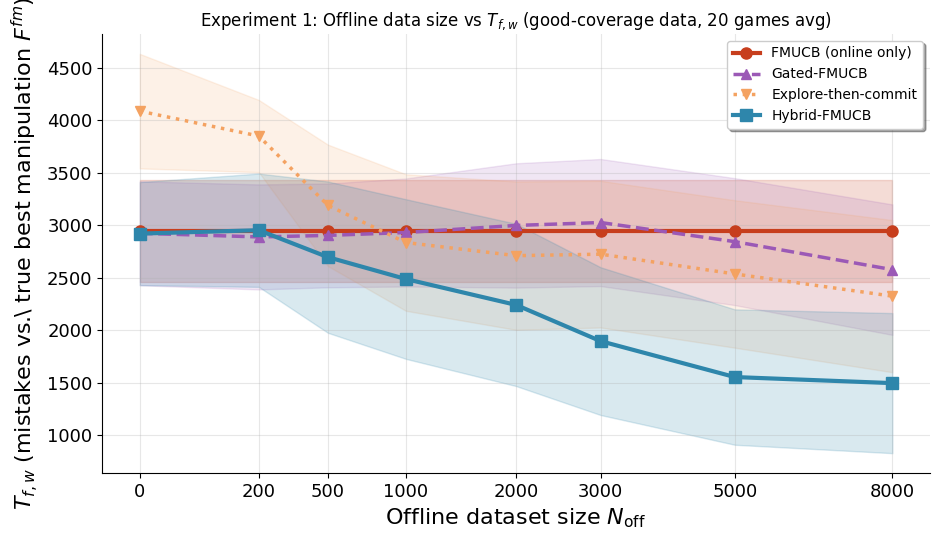
\includegraphics[width=.8\linewidth]{figures/exp1_noff_vs_tfw.png}
    \caption{$T_{f,w}$ vs.\ $N_{\mathrm{off}}$ under good coverage, $4\times 4$ games (20 games $\times$ 24 seeds). Shaded bands: 95\% CIs.}
    \label{fig:exp1-noff-vs-tfw}
\end{figure}
\begin{figure}[H]
    \centering
    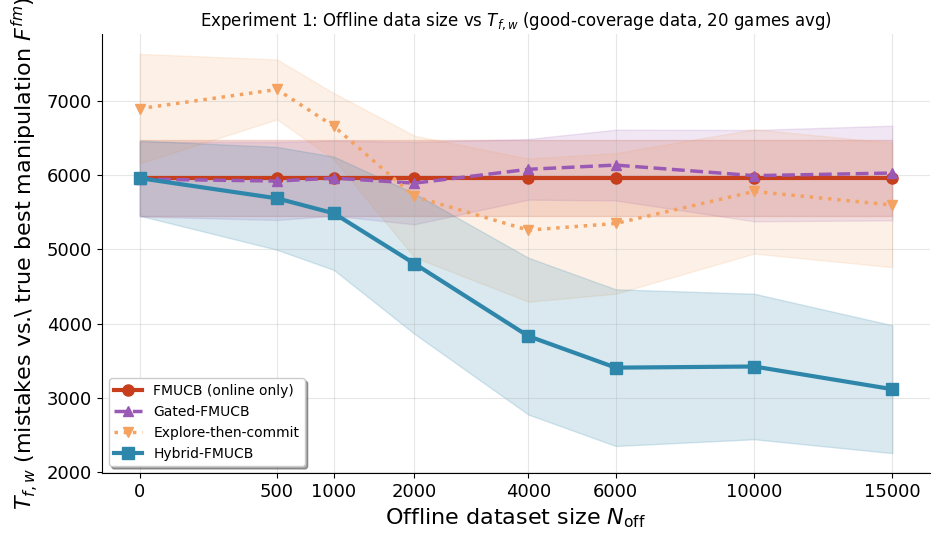
\includegraphics[width=.8\linewidth]{figures/exp1_noff_vs_tfw_6x6.png}
    \caption{Same as Figure~\ref{fig:exp1-noff-vs-tfw} for $6\times 6$ games.}
    \label{fig:exp1-noff-6x6}
\end{figure}
\begin{figure}[H]
    \centering
    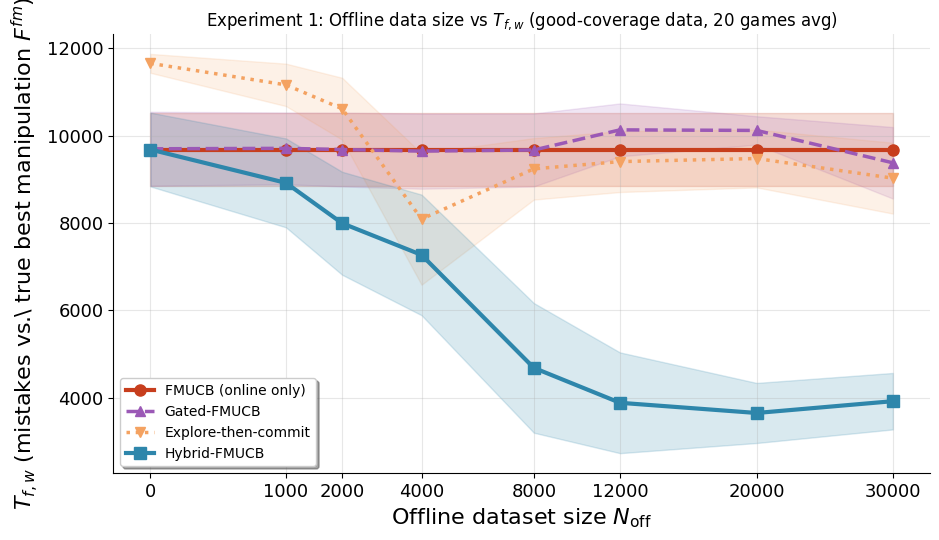
\includegraphics[width=.8\linewidth]{figures/exp1_noff_vs_tfw_8x8.png}
    \caption{Same as Figure~\ref{fig:exp1-noff-vs-tfw} for $8\times 8$ games.}
    \label{fig:exp1-noff-8x8}
\end{figure}

Figures~\ref{fig:exp1-noff-vs-tfw}--\ref{fig:exp1-noff-8x8} show a consistent pattern across all three game sizes: Hybrid-FMUCB decreases monotonically with $N_{\mathrm{off}}$, while the FMUCB baseline remains flat. The relative reduction grows with game size---approximately $50\%$ for $4\times 4$, $48\%$ for $6\times 6$, and $60\%$ for $8\times 8$---indicating that larger action spaces benefit more from offline data, as there are more manipulation-relevant cells whose coverage reduces online exploration. ETC starts high (committing to poorly estimated rules at low $N_{\mathrm{off}}$) and improves but remains above Hybrid throughout. Gated-FMUCB tracks the online baseline because the formal certificate rarely passes: games with small $\Delta_3$ never satisfy the transfer condition, forcing Gated to discard all offline data. Hybrid wins because it softly integrates offline data into shrinking confidence sets, benefiting from partial information without requiring the formal certificate to pass.

\paragraph{Coverage quality.}
We fix $N_{\mathrm{off}}$ at a moderate level scaled to game size ($1000$ for $4\times 4$, $2000$ for $6\times 6$, $4000$ for $8\times 8$) and compare three offline data distributions: good coverage (60\% on manipulation-relevant cells $(a, F_{\mathrm{fm}}(a))$, 20\% on follower best-response cells, 20\% uniform), neutral (uniform across all $|\cA||\cB|$ cells), and adversarial (90\% on non-manipulation cells, 10\% sparse uniform).
\begin{figure}[H]
    \centering
    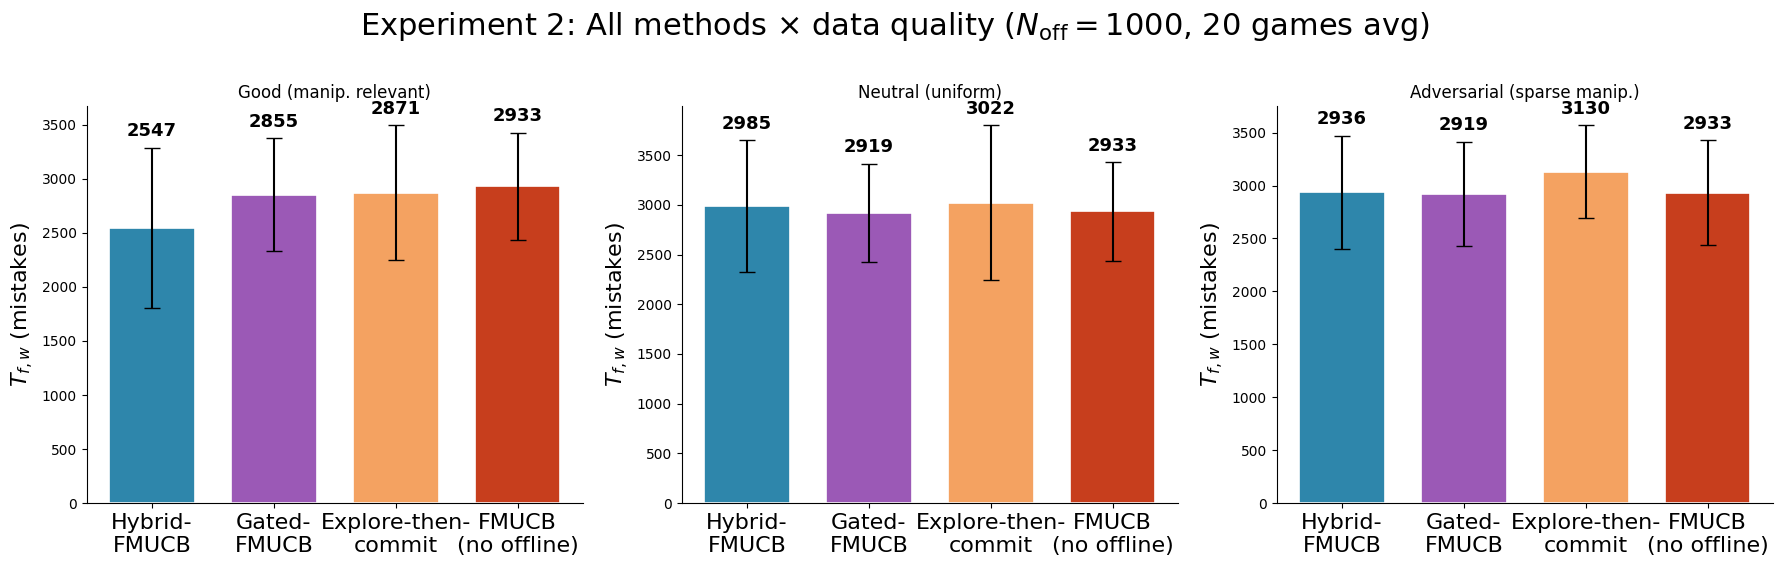
\includegraphics[width=.92\linewidth]{figures/exp2_coverage_bars.png}
    \caption{$T_{f,w}$ across four methods and three coverage regimes, $4\times 4$ games, $N_{\mathrm{off}}=1000$.}
    \label{fig:exp2-coverage}
\end{figure}
\begin{figure}[H]
    \centering
    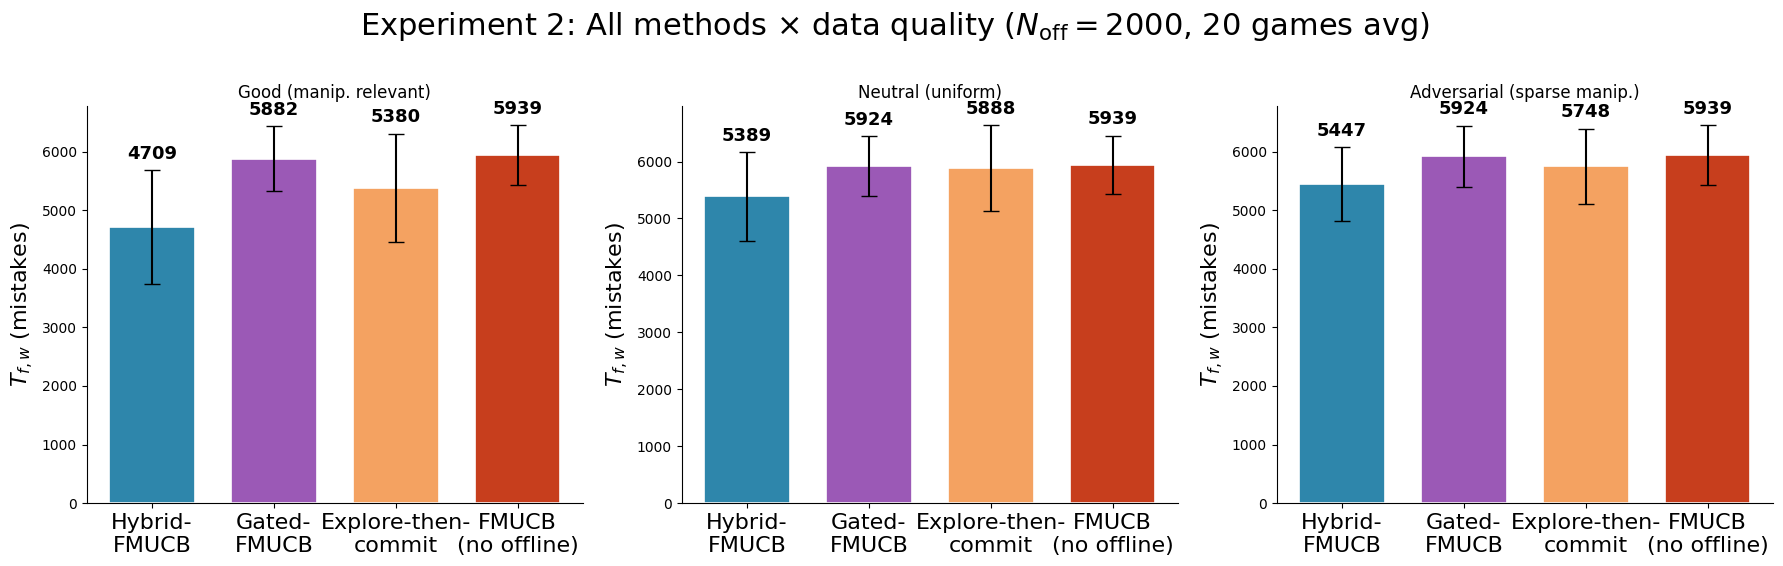
\includegraphics[width=.92\linewidth]{figures/exp2_coverage_bars_6x6.png}
    \caption{Same as Figure~\ref{fig:exp2-coverage} for $6\times 6$ games, $N_{\mathrm{off}}=2000$.}
    \label{fig:exp2-coverage-6x6}
\end{figure}
\begin{figure}[H]
    \centering
    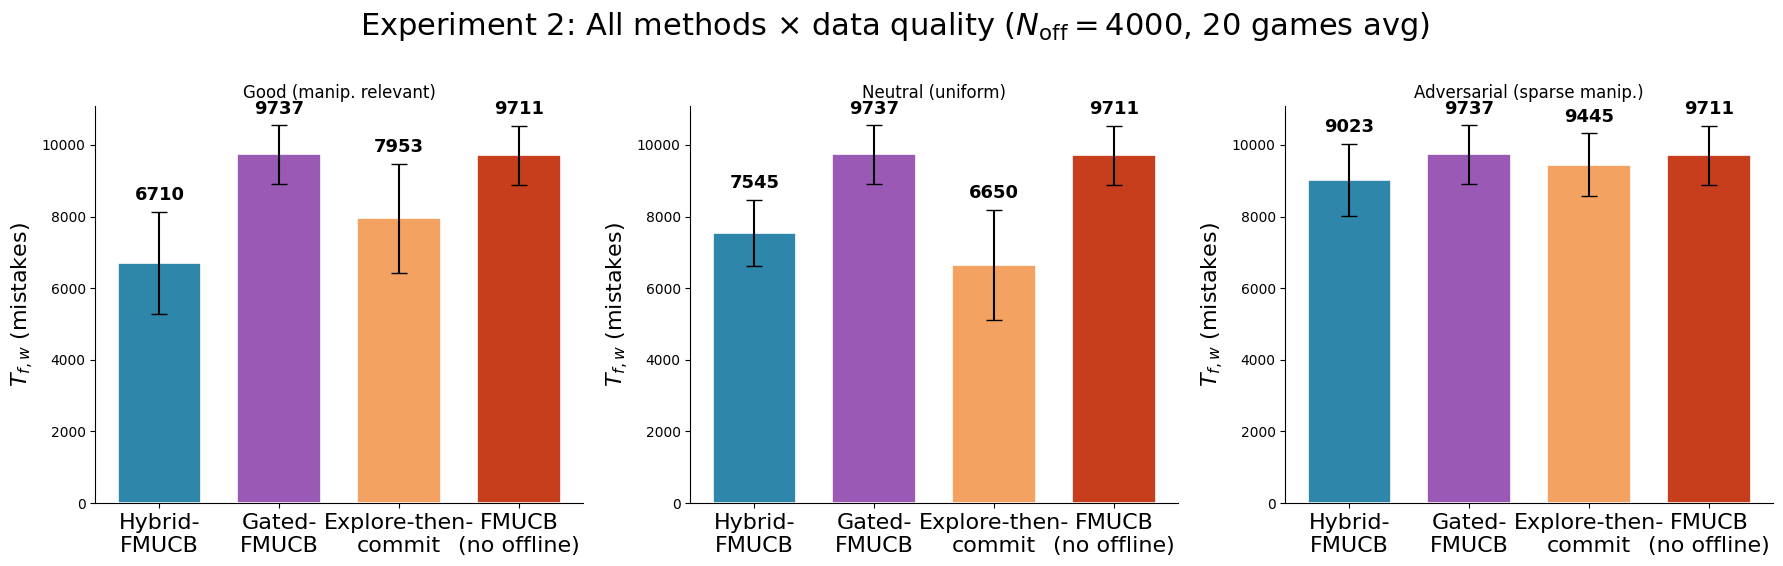
\includegraphics[width=.92\linewidth]{figures/exp2_coverage_bars_8x8.png}
    \caption{Same as Figure~\ref{fig:exp2-coverage} for $8\times 8$ games, $N_{\mathrm{off}}=4000$.}
    \label{fig:exp2-coverage-8x8}
\end{figure}
Figures~\ref{fig:exp2-coverage}--\ref{fig:exp2-coverage-8x8} reveal how each method responds to data quality across game sizes. Under good coverage, Hybrid-FMUCB achieves a clear reduction relative to the FMUCB baseline, and the advantage scales with game size: $13\%$ for $4\times 4$, $21\%$ for $6\times 6$, and $31\%$ for $8\times 8$. This scaling is predicted by the theory: in larger games, the manipulation contrast depends on more cells, so good coverage of those cells provides proportionally greater information gain.

Under neutral coverage, an interesting pattern emerges in the $8\times 8$ setting: ETC ($T_{f,w}\approx 6650$) outperforms Hybrid-FMUCB ($\approx 7545$). This is consistent with the theory---with $N_{\mathrm{off}}=4000$ spread uniformly over $64$ cells, ETC receives $\approx 62$ samples per cell, sufficient for accurate estimation. When offline estimates are already reliable, ETC's commit-then-play strategy avoids the exploration overhead inherent in confidence-set maintenance, gaining an advantage. This regime corresponds to moderate $C^{\mathrm{man}}$ under uniform data: the offline signal is informative enough that immediate commitment outperforms continued exploration. Under adversarial coverage, all hybrid methods perform close to the online baseline, confirming that Hybrid-FMUCB degrades gracefully---its online phase corrects misleading offline signals rather than committing to them.

These results validate the $C^{\mathrm{man}}$ theory: the value of offline data depends on whether it covers the manipulation-relevant comparisons, not its nominal size. When $C^{\mathrm{man}}$ is small (good coverage), Hybrid-FMUCB benefits most; when $C^{\mathrm{man}}$ is effectively infinite (adversarial), the online phase ensures no harm.

\paragraph{Contextual generalization.}
We use an affine Kronecker feature map $\phi(x,a,b)=[1;\,z_x\otimes[e_a;\,e_b]]\in\R^{25}$ with $d_{\mathrm{ctx}}=3$-dimensional context embeddings, $|\cA|=|\cB|=4$, and $N_{\mathrm{off}}=1000$, sweeping $|\cX|\in\{5,10,20,30\}$. Because the additive Kronecker structure makes the worst response $\mathrm{wr}(a)=\arg\min_b\mu_\ell(x,a,b)$ independent of context $x$ (the context scaling is common across $b$), this is a simplification relative to the general contextual setting where $\mathrm{wr}(a)$ could vary with $x$. Algorithm~\ref{alg:contextual-hybrid-fmucb} pools all offline samples into one $25$-dimensional ridge regression; the tabular baseline runs Algorithm~\ref{alg:hybrid-fmucb-fclass} independently per context.
\begin{figure}[t]
    \centering
    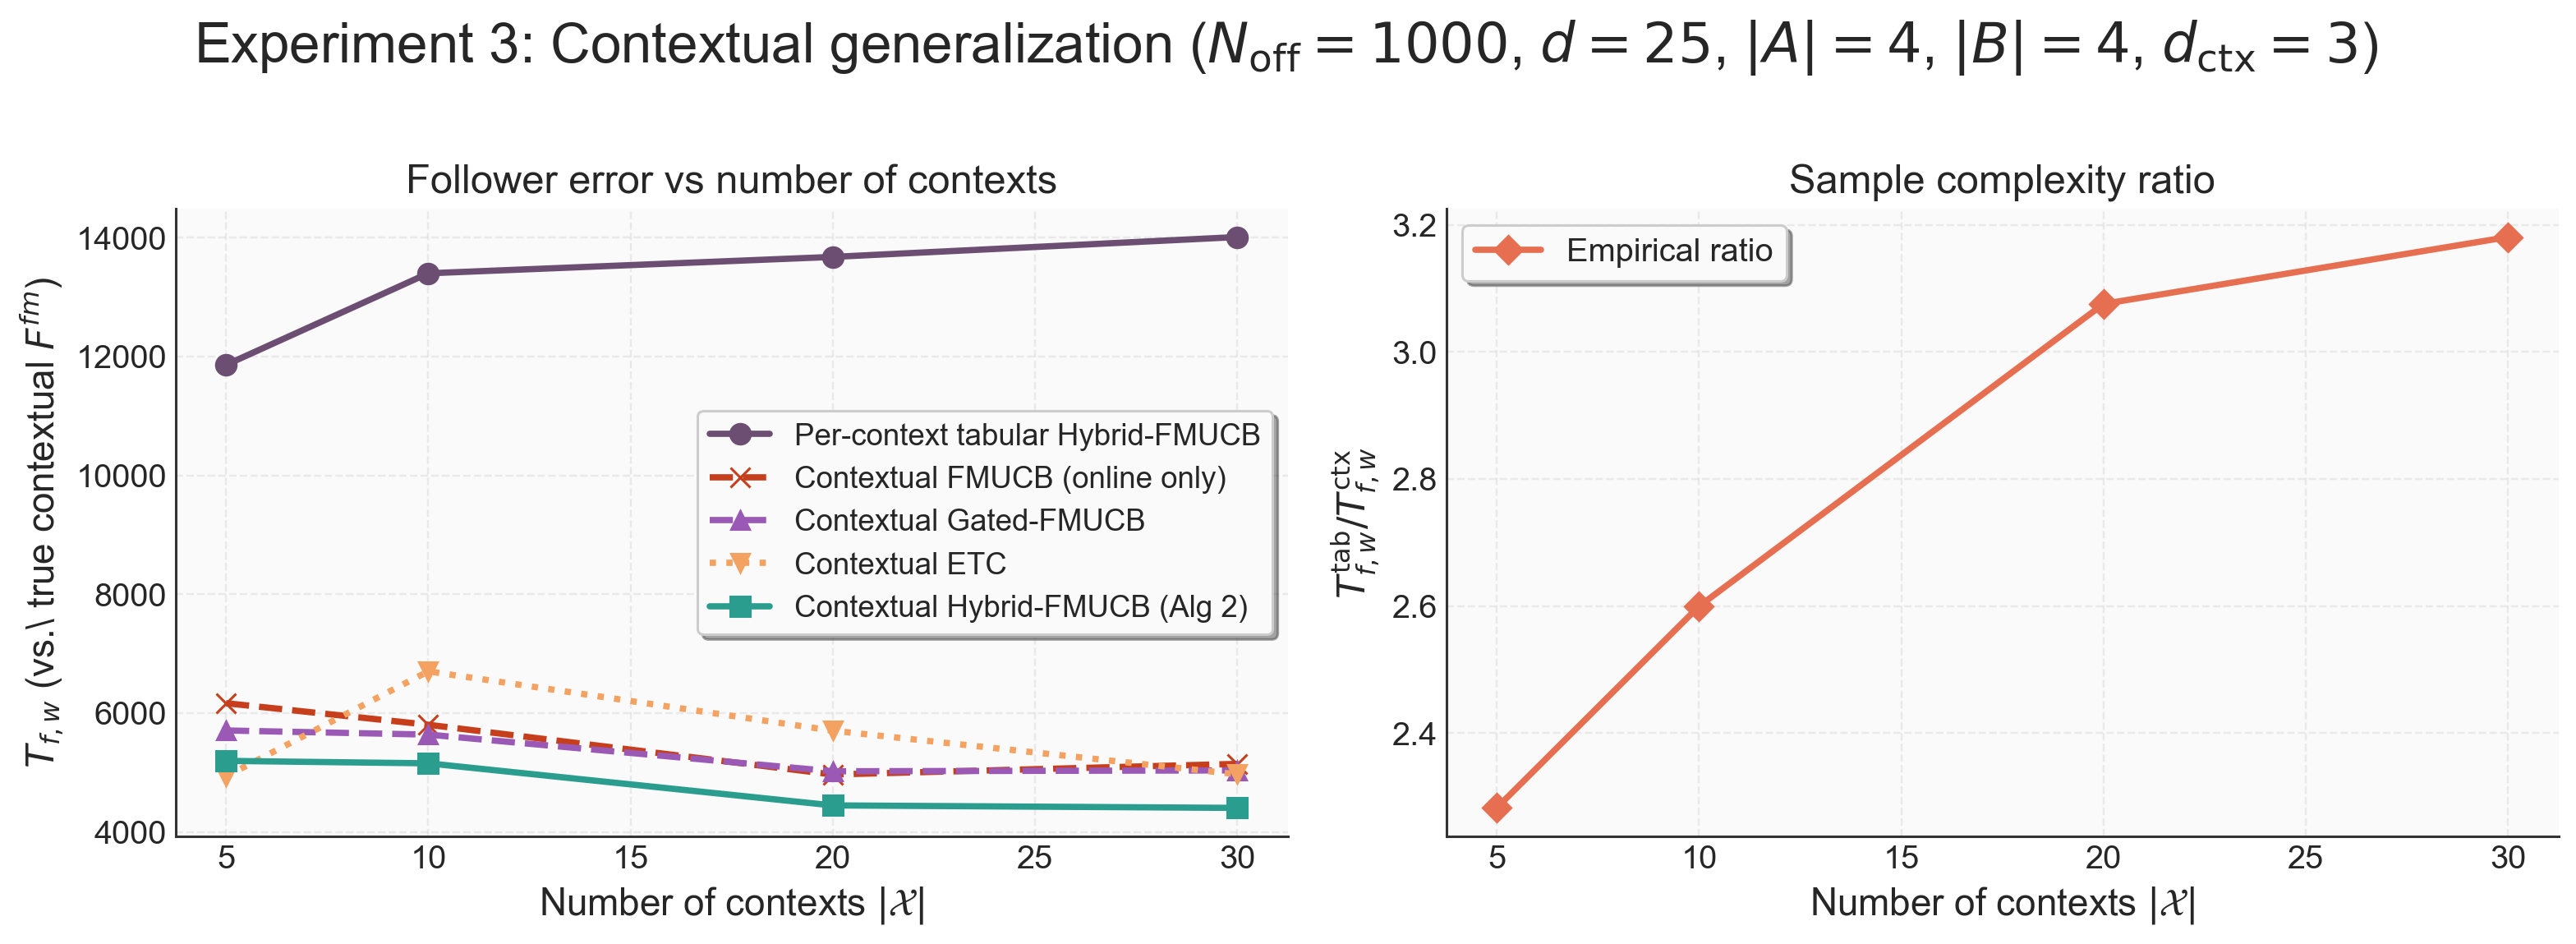
\includegraphics[width=1\linewidth]{figures/exp3_contextual_vs_tabular.png}
    \caption{Contextual vs.\ per-context tabular Hybrid-FMUCB as $|\cX|$ grows. Right: empirical ratio $T_{f,w}^{\mathrm{tab}}/T_{f,w}^{\mathrm{ctx}}$.}
    \label{fig:exp3-contextual}
\end{figure}
Figure~\ref{fig:exp3-contextual} shows tabular failures rising from $\approx 11{,}800$ at $|\cX|=5$ to $\approx14{,}000$ at $|\cX|=30$ as the per-context offline budget thins, while the contextual method stays near ${\approx}5{,}300$ and slightly decreases with more contexts (more data for the shared $\theta^\star$). The empirical ratio grows from $2.2$ to $3.2$, consistent with the qualitative prediction of Corollary~\ref{cor:contextual-tabular-sep} that contextual pooling becomes increasingly advantageous as $|\cX|$ grows relative to $d$.

\section{Discussion and Conclusion}
\label{sec:discussion}
We introduced a hybrid offline-online framework for follower manipulation in repeated general-sum Stackelberg bandits. The coefficient $C^{\mathrm{man}}$ formalizes the same principle that drives Hybrid RL~\cite{song2022hybrid}: offline data is useful when it constrains the decision-relevant directions, not necessarily when it provides uniform coverage. Hybrid-FMUCB leverages this fact to certify the leader-side feasibility of target manipulations at initialization when offline transfer is sufficient, and otherwise uses online interaction to resolve the remaining ambiguity. The contextual extension shows that the same transfer-plus-elimination logic applies when rewards share a low-dimensional structure across contexts, replacing independent per-context tabular estimation with a pooled regression problem.

Because the paper studies manipulation as an algorithmic object, the results are dual-use: they can inform defenses against strategic followers, but they may also help characterize when manipulation is statistically feasible. For this reason, our experiments are synthetic and our discussion emphasizes certification, detection, and leader-side defenses rather than deployment guidance.

Several directions remain open. Our theory assumes realizability; agnostic and misspecified settings are important for practice. The contextual analysis uses linear features; extending the framework to richer nonparametric or neural classes would require new confidence and transfer arguments. Finally, the leader side deserves further study: a hybrid leader may use offline data not only to learn faster, but also to detect or defend against manipulation. Extending these ideas to multi-step Stackelberg Markov games would connect the framework even more directly to hybrid reinforcement learning.

\bibliographystyle{abbrvnat}
\bibliography{references}
\newpage
\appendix
\section{Related Work}\label{sec:related}

\paragraph{Decentralized learning in games.}
Decentralized no-regret learning in general-sum simultaneous games converges to coarse correlated equilibria~\cite{blum2007external}, a result sharpened by optimistic methods~\cite{daskalakis2021near, chen2020hedging, anagnostides2022near} and extended to Markov games~\cite{jin2021v, liu2021sharp}. A broad literature studies variants of this problem~\cite{wu2022multi, meng2021decentralized, wei2021last, song2021can, mao2023provably, zhong2023can, ghosh2023provably}. We focus on Stackelberg (sequential) rather than simultaneous games, where the asymmetric timing creates qualitatively different strategic incentives.

\paragraph{Learning in Stackelberg games.}
Stackelberg games arise in security~\cite{tambe2011security, gan2018stackelberg}, auctions~\cite{myerson1981optimal, cole2014sample}, taxation~\cite{zheng2020ai}, mechanism design~\cite{conitzer2002complexity}, and autonomous driving~\cite{shalev2016safe}; see~\cite{roughgarden2010algorithmic} for background. Most learning results assume the leader's perspective with access to a follower best-response oracle~\cite{blum2014learning, peng2019learning, balcan2015commitment, letchford2009learning}. Recent work studies two-player learning under specific reward structures: zero-sum~\cite{goktas2022zero, sun2023zero} and cooperative~\cite{kao2022decentralized, zhao2023online}. We study general-sum games without structural reward assumptions, following Bai et al.~\cite{bai2021sample} (centralized) and Yu and Chen~\cite{yu2024decentralized} (decentralized online). Our contribution is extending the latter to the hybrid offline-online setting with function approximation.

\paragraph{Follower manipulation.}
The leader's first-mover advantage in Stackelberg equilibria~\cite{von2010leadership} relies on the follower best-responding truthfully. A line of work shows that a strategic follower can instead manipulate a commitment leader by misreporting payoffs, inducing a follower-preferred outcome~\cite{gan2019manipulating, gan2019imitative, nguyen2019imitative, birmpas2020optimally, chen2025optimal, chen2023learning}. These results are offline and single-player. Yu and Chen~\cite{yu2024decentralized} extend manipulation to online learning with noisy bandit feedback and prove last-iterate convergence against EXP3 and UCBE leaders. We further extend to the hybrid setting where offline historical data supplements online interaction.

\paragraph{Hybrid offline-online RL.}
Hybrid RL leverages both offline data and online interaction to overcome the coverage limitations of purely offline learning~\cite{song2022hybrid, wagenmaker2023leveraging, li2023reward, ball2023efficient, ren2024hybrid}. The central insight is that offline data need not cover the full state-action space; it suffices to cover the decision-relevant directions, as captured by the Bellman-error transfer coefficient~\cite{song2022hybrid}. Our $C^{\mathrm{man}}$ is the Stackelberg analogue: it measures whether offline prediction accuracy on $\nu$ implies accurate manipulation-contrast estimates. This reflects a broader principle -- also observed in post-training~\cite{chen2025coverage} -- that global estimation accuracy is insufficient for downstream performance; what matters is coverage of the regions that control the target decision.

\section{Proof of Theorem~\ref{thm:hybrid-cman-exp3}}
\label{app:proof-main}

\begin{proof}[Proof of Theorem~\ref{thm:hybrid-cman-exp3}]
Fix the true best manipulation rule $F_{\mathrm{fm}}$ associated with
the target action $a_{\mathrm{fm}}$, and define the induced leader
reward
\[
\mu_m(a):=\mu_\ell(a,F_{\mathrm{fm}}(a)).
\]
By definition of the best manipulation,
\[
a_{\mathrm{fm}}\in\arg\max_{a\in\mathcal A}\mu_m(a),
\qquad
\Delta_3
=
\mu_m(a_{\mathrm{fm}})
-
\max_{a\neq a_{\mathrm{fm}}}\mu_m(a)
>0.
\]

We split the proof into offline certification, elimination of
incorrect manipulations, and the leader-side decomposition. The key
difference from the tabular proof of \cite{yu2024decentralized} is
that the hybrid argument contains an explicit offline transfer step:
rather than beginning directly from online confidence radii, we first
use the offline dataset to certify that the target manipulation is
already feasible at initialization. After that point, the rest of the
argument follows the same three-part elimination logic as in the FMUCB
analysis of \cite{yu2024decentralized}, namely elimination of wrong
worst responses, infeasible manipulations, and feasible but
follower-suboptimal manipulations.

\paragraph{Step 1: Offline certification via the qualified-manipulation coefficient.}
Recall that for any candidate manipulation $(F,a^\star)$, the
qualified-manipulation transfer coefficient
$C^{\mathrm{man}}(F,a^\star)$ controls how offline prediction error
under the behavior distribution $\nu$ transfers to error in the
manipulation contrast:
\[
\bigl|
\Delta_{F,a^\star}(\widehat g)-\Delta_{F,a^\star}(\mu_\ell)
\bigr|
\le
C^{\mathrm{man}}(F,a^\star)
\sqrt{\E_\nu\!\left[(\widehat g-\mu_\ell)^2\right]}.
\]
Apply this with $(F,a^\star)=(F_{\mathrm{fm}},a_{\mathrm{fm}})$ and
$\widehat g=\widehat g_{\ell,0}$, the leader-side estimator built from
the offline data. By the offline transfer assumption,
\[
C^{\mathrm{man}}(F_{\mathrm{fm}},a_{\mathrm{fm}})
\sqrt{\E_\nu\!\left[(\widehat g_{\ell,0}-\mu_\ell)^2\right]}
\le
\frac{\Delta_3}{4}.
\]
Therefore,
\[
\bigl|
\Delta_{F_{\mathrm{fm}},a_{\mathrm{fm}}}(\widehat g_{\ell,0})
-
\Delta_{F_{\mathrm{fm}},a_{\mathrm{fm}}}(\mu_\ell)
\bigr|
\le
\frac{\Delta_3}{4}.
\]
Since
\[
\Delta_{F_{\mathrm{fm}},a_{\mathrm{fm}}}(\mu_\ell)
=
\mu_m(a_{\mathrm{fm}})
-
\max_{a\neq a_{\mathrm{fm}}}\mu_m(a)
=
\Delta_3,
\]
it follows that
\[
\Delta_{F_{\mathrm{fm}},a_{\mathrm{fm}}}(\widehat g_{\ell,0})
\ge
\Delta_3-\frac{\Delta_3}{4}
=
\frac{3\Delta_3}{4}
>0.
\]

Now work on the confidence event under which
$\mu_\ell\in\mathcal G_{\ell,0}$. By construction of the initial
confidence set, every $g\in\mathcal G_{\ell,0}$ is statistically
indistinguishable from $\widehat g_{\ell,0}$ up to the prescribed
confidence tolerance. Equivalently, the confidence class has been
chosen so that the leader-side contrast uncertainty at time $0$ is
controlled by the same offline estimation error, and therefore for
every $g\in\mathcal G_{\ell,0}$,
\[
\bigl|
\Delta_{F_{\mathrm{fm}},a_{\mathrm{fm}}}(g)
-
\Delta_{F_{\mathrm{fm}},a_{\mathrm{fm}}}(\mu_\ell)
\bigr|
\le
\frac{\Delta_3}{4}.
\]
Hence
\[
\Delta_{F_{\mathrm{fm}},a_{\mathrm{fm}}}(g)
\ge
\Delta_{F_{\mathrm{fm}},a_{\mathrm{fm}}}(\mu_\ell)-\frac{\Delta_3}{4}
=
\Delta_3-\frac{\Delta_3}{4}
=
\frac{3\Delta_3}{4}
>0.
\]
Since this holds for every $g\in\mathcal G_{\ell,0}$,
\[
\inf_{g\in\mathcal G_{\ell,0}}
\Delta_{F_{\mathrm{fm}},a_{\mathrm{fm}}}(g)>0,
\]
so the true target manipulation is already certifiably feasible from
offline data alone.

This is exactly the point at which the hybrid proof differs from the
purely online proof of \cite{yu2024decentralized}. In the theorem of
\cite{yu2024decentralized}, feasibility is established only after
sufficient online exploration shrinks the tabular confidence radii. In
the present theorem, the coefficient $C^{\mathrm{man}}$ allows the
offline data to certify the target manipulation before any online
interaction occurs.

\paragraph{Step 2: Elimination of wrong worst responses.}
Consider any leader action $a$ and any follower action
$b\neq \mathrm{wr}(a)$. By definition of $\Delta_5$,
\[
\mu_\ell(a,b)-\mu_\ell(a,\mathrm{wr}(a))\ge \Delta_5.
\]
Equivalently, the manipulation contrast associated with replacing the
true worst response $\mathrm{wr}(a)$ by $b$ is separated from zero by
at least $\Delta_5$.

Suppose now that the leader-side uncertainty has shrunk to the regime
\[
\omega_{\ell,t}(F,a)\le \frac{\Delta_5}{4}
\]
for every response rule $F$ relevant to this comparison. Then for any
such $F$ and any $g\in\mathcal G_{\ell,t}$,
\[
\bigl|
\Delta_{F,a}(g)-\Delta_{F,a}(\mu_\ell)
\bigr|
\le
\omega_{\ell,t}(F,a)
\le
\frac{\Delta_5}{4}.
\]
Since the true ordering gap is at least $\Delta_5$, the confidence set
is too narrow to reverse the ordering between $b$ and
$\mathrm{wr}(a)$. To see this, consider two response rules $F_b$ and $F_w$ that agree
on every $a'\neq a$: $F_b(a)=b$ and $F_w(a)=\mathrm{wr}(a)$. Both target $a^\star=a$. Their contrasts
share the same $\max$ term, so for any $g\in\mathcal G_{\ell,t}$,
\[
\Delta_{F_b,a}(g)-\Delta_{F_w,a}(g)
=g(a,b)-g(a,\mathrm{wr}(a)).
\]
The same identity holds at $\mu_\ell$. Since
$\omega_{\ell,t}\le\Delta_5/4$ for every response rule,
\begin{align*}
\bigl|[g(a,b)-g(a,\mathrm{wr}(a))]
-[\mu_\ell(a,b)-\mu_\ell(a,\mathrm{wr}(a))]\bigr|
&\le
\omega_{\ell,t}(F_b,a)+\omega_{\ell,t}(F_w,a)
\le \frac{\Delta_5}{2}.
\end{align*}
Therefore $g(a,b)-g(a,\mathrm{wr}(a))\ge \Delta_5-\Delta_5/2
=\Delta_5/2>0$, so every $g\in\mathcal G_{\ell,t}$ preserves
the identity of the worst response, and wrong worst-response
identification can no longer persist.

By definition of the sample-complexity function, this regime is
reached after time $\tau_\ell(\Delta_5/4)$. Because the leader uses
EXP3 with exploration parameter $\alpha$, each leader action is
sampled with probability at least $\alpha/A$ on every round. Thus the
number of rounds needed to accumulate
$\tau_\ell(\Delta_5/4)$ effective samples for a fixed action $a$ is of
order
\[
O\!\left(\frac{A}{\alpha}\tau_\ell\!\left(\frac{\Delta_5}{4}\right)\right).
\]
Summing over all $a\in\mathcal A$ yields the contribution
\[
O\!\left(
\frac{A^2}{\alpha}\tau_\ell\!\left(\frac{\Delta_5}{4}\right)
\right).
\]

This is the direct function-class counterpart of the first elimination
term in \cite{yu2024decentralized}: the structure of the argument is
the same, but the entrywise tabular confidence radius is replaced by
decision-relevant uncertainty of the function-class confidence set.

\paragraph{Step 3: Elimination of infeasible manipulation candidates.}
Now consider any pair $(F,a)$ that is infeasible under the true leader
reward, meaning
\[
\Delta_{F,a}(\mu_\ell)\le -\Delta_6.
\]
Suppose that at time $t$,
\[
\omega_{\ell,t}(F,a)\le \frac{\Delta_6}{4}.
\]
Then for every $g\in\mathcal G_{\ell,t}$,
\[
\Delta_{F,a}(g)
\le
\Delta_{F,a}(\mu_\ell)+\omega_{\ell,t}(F,a)
\le
-\Delta_6+\frac{\Delta_6}{4}
=
-\frac{3\Delta_6}{4}
<0.
\]
Hence $(F,a)$ cannot satisfy
\[
\inf_{g\in\mathcal G_{\ell,t}}\Delta_{F,a}(g)>0,
\]
and therefore cannot belong to the feasible set
\[
\mathcal M_t
=
\{(F,a):\inf_{g\in\mathcal G_{\ell,t}}\Delta_{F,a}(g)>0\}.
\]
Thus every infeasible manipulation is removed from consideration once
the leader-side contrast uncertainty falls below $\Delta_6/4$. By
definition, this occurs after time $\tau_\ell(\Delta_6/4)$.

As above, the EXP3 exploration lower bound implies that collecting the
required evidence for a fixed candidate costs
\[
O\!\left(
\frac{A}{\alpha}\tau_\ell\!\left(\frac{\Delta_6}{4}\right)
\right)
\]
rounds. Summing over the $AB$ candidate manipulation pairs yields the
contribution
\[
O\!\left(
\frac{A^2B}{\alpha}\tau_\ell\!\left(\frac{\Delta_6}{4}\right)
\right).
\]

This is the second analogue of the elimination proof in
\cite{yu2024decentralized}: again the logical structure is identical,
but in the hybrid theorem the cost is only the \emph{residual} online
cost left after the offline dataset has already shrunk the confidence
class.

\paragraph{Step 4: Elimination of follower-suboptimal feasible pairs.}
Consider now a feasible manipulation $(F,a)$ that is nevertheless
suboptimal for the follower. By definition of $\Delta_4$,
\[
\mu_f(a_{\mathrm{fm}},F_{\mathrm{fm}}(a_{\mathrm{fm}}))
-
\mu_f(a,F(a))
\ge
\Delta_4.
\]
Assume that the follower-side uncertainty has shrunk so that
\[
\omega_{f,t}(F,a)\le \frac{\Delta_4}{4}
\qquad\text{and}\qquad
\omega_{f,t}(F_{\mathrm{fm}},a_{\mathrm{fm}})\le \frac{\Delta_4}{4}.
\]
Then for every $h\in\mathcal G_{f,t}$,
\[
\bigl|
h(a,F(a))-\mu_f(a,F(a))
\bigr|
\le
\frac{\Delta_4}{4},
\]
and similarly
\[
\bigl|
h(a_{\mathrm{fm}},F_{\mathrm{fm}}(a_{\mathrm{fm}}))
-
\mu_f(a_{\mathrm{fm}},F_{\mathrm{fm}}(a_{\mathrm{fm}}))
\bigr|
\le
\frac{\Delta_4}{4}.
\]
Therefore the optimistic value that the follower can assign to the
suboptimal pair $(F,a)$ exceeds its true value by at most
$\Delta_4/4$, while the pessimistic value of the true best feasible
manipulation falls short of its true value by at most $\Delta_4/4$.
Using the true gap $\Delta_4$, we obtain
\begin{align*}
\sup_{h\in\mathcal G_{f,t}} h(a,F(a))
&\le
\mu_f(a,F(a))+\frac{\Delta_4}{4} \\
&\le
\mu_f(a_{\mathrm{fm}},F_{\mathrm{fm}}(a_{\mathrm{fm}}))
-\Delta_4+\frac{\Delta_4}{4} \\
&=
\mu_f(a_{\mathrm{fm}},F_{\mathrm{fm}}(a_{\mathrm{fm}}))
-\frac{3\Delta_4}{4},
\end{align*}
whereas
\begin{align*}
\inf_{h\in\mathcal G_{f,t}}
h(a_{\mathrm{fm}},F_{\mathrm{fm}}(a_{\mathrm{fm}}))
&\ge
\mu_f(a_{\mathrm{fm}},F_{\mathrm{fm}}(a_{\mathrm{fm}}))
-\frac{\Delta_4}{4}.
\end{align*}
Hence the optimistic value of $(F,a)$ can no longer dominate the
pessimistic value of the true best feasible manipulation, and so
$(F,a)$ cannot be selected by the algorithm after time
$\tau_f(\Delta_4/4)$.

Summing this contribution over the feasible candidates gives
\[
O\!\left(
\frac{A^2B}{\alpha}\tau_f\!\left(\frac{\Delta_4}{4}\right)
\right).
\]

This is the third and final elimination component paralleling the
proof of \cite{yu2024decentralized}: the follower no longer chooses an
incorrect feasible pair once the confidence class is too narrow to
mask the suboptimality gap.

\paragraph{Step 5: Total follower failure bound.}
Every round in which the follower fails to play the true best
manipulation must be attributable to one of the three error types
above:
\begin{enumerate}
    \item misidentification of the worst response for some leader
    action;
    \item failure to eliminate an infeasible manipulation candidate;
    \item failure to eliminate a feasible but follower-suboptimal
    manipulation.
\end{enumerate}
The first type contributes at most
\[
O\!\left(
\frac{A^2}{\alpha}\tau_\ell\!\left(\frac{\Delta_5}{4}\right)
\right),
\]
the second contributes at most
\[
O\!\left(
\frac{A^2B}{\alpha}\tau_\ell\!\left(\frac{\Delta_6}{4}\right)
\right),
\]
and the third contributes at most
\[
O\!\left(
\frac{A^2B}{\alpha}\tau_f\!\left(\frac{\Delta_4}{4}\right)
\right).
\]
Combining the three terms and incorporating the standard
$\log(1/\delta)$ overhead from the EXP3-to-last-iterate reduction
yields
\[
T_{f,w}
\le
O\!\left(
\frac{A}{\alpha}\log\frac1\delta
\left[
A\,\tau_\ell\!\left(\frac{\Delta_5}{4}\right)
+
AB\,\tau_\ell\!\left(\frac{\Delta_6}{4}\right)
+
AB\,\tau_f\!\left(\frac{\Delta_4}{4}\right)
\right]
\right),
\]
which is exactly the desired follower-failure bound.

Relative to \cite{yu2024decentralized}, the form of this bound is the
same at the level of decomposition: three elimination terms, each tied
to a structural gap. The difference is that in the hybrid setting the
online quantities $\tau_\ell(\cdot)$ and $\tau_f(\cdot)$ represent
only the residual sample complexity after incorporating the offline
dataset through the transfer step in Step~1.

\paragraph{Step 6: Leader-side decomposition.}
It remains to convert the follower failure bound into the leader-side
regret decomposition. The argument is the same corruption-style
reduction used in the noisy FMUCB proof.

For any $a\neq a_{\mathrm{fm}}$,
\begin{align*}
\sum_{t=1}^T \bigl(r_t(a)-r_t(a_{\mathrm{fm}})\bigr)
&=
\sum_{t=1}^T \bigl(r_t(a)-\mu_m(a)\bigr)
+
\sum_{t=1}^T \bigl(\mu_m(a)-\mu_m(a_{\mathrm{fm}})\bigr)
+
\sum_{t=1}^T \bigl(\mu_m(a_{\mathrm{fm}})-r_t(a_{\mathrm{fm}})\bigr).
\end{align*}
The middle term is nonpositive and in fact bounded above by
\[
\sum_{t=1}^T \bigl(\mu_m(a)-\mu_m(a_{\mathrm{fm}})\bigr)
\le
-\Delta_3 T,
\]
because
\[
\mu_m(a)-\mu_m(a_{\mathrm{fm}})\le -\Delta_3
\qquad\text{for all }a\neq a_{\mathrm{fm}}.
\]
Thus, if the follower were always to play the manipulation rule
$F_{\mathrm{fm}}$, the leader would face a stationary bandit problem
with mean rewards $\mu_m(a)$, and the regret analysis would reduce to
that benchmark alone.

The only discrepancy from that stationary benchmark comes from the
rounds in which the follower does \emph{not} play the true best
manipulation. Partition $\{1,\dots,T\}$ into
$\cT_{\mathrm{ok}}:=\{t:b_t=F_{\mathrm{fm}}(a_t)\}$ and
$\cT_{\mathrm{fail}}:=\{1,\dots,T\}\setminus\cT_{\mathrm{ok}}$,
so $|\cT_{\mathrm{fail}}|\le T_{f,w}$. Write the leader-side
regret against the manipulation benchmark as
\[
R(T)
=\sum_{t=1}^T\bigl[\mu_m(a_{\mathrm{fm}})-\mu_\ell(a_t,b_t)\bigr].
\]
On any clean round $t\in\cT_{\mathrm{ok}}$,
$b_t=F_{\mathrm{fm}}(a_t)$, so
$\mu_\ell(a_t,b_t)=\mu_m(a_t)$ and the instantaneous regret
$\mu_m(a_{\mathrm{fm}})-\mu_m(a_t)$ is exactly that of a stationary
bandit with means $\mu_m(a)$. On any failure round
$t\in\cT_{\mathrm{fail}}$, the follower plays some
$b_t\neq F_{\mathrm{fm}}(a_t)$, so the instantaneous regret
$\mu_m(a_{\mathrm{fm}})-\mu_\ell(a_t,b_t)$ can differ from the
stationary benchmark by at most $1$ (since rewards lie in $[0,1]$).
Therefore
\[
R(T)
\le
\underbrace{\sum_{t\in\cT_{\mathrm{ok}}}
\bigl[\mu_m(a_{\mathrm{fm}})-\mu_m(a_t)\bigr]}_{=\;R_{\mathrm{leader}}(|\cT_{\mathrm{ok}}|;\,\mu_m)}
+\;T_{f,w}.
\]
Since $R_{\mathrm{leader}}(|\cT_{\mathrm{ok}}|;\mu_m)\le R_{\mathrm{leader}}(T;\mu_m)$
and concentrating the observed rewards around their means adds an
$O(\sqrt{T\log(1/\delta)})$ high-probability term, the overall bound
is
\[
R(T) \le R_{\mathrm{leader}}(T;\mu_m) + T_{f,w} + O\left(\sqrt{T\log\tfrac{1}{\delta}}\right),
\]
which is the claimed bound.

This completes the proof.
\end{proof}


\section{Proof of Theorem~\ref{thm:hybrid-contextual-sample-complexity}}
\label{app:proof-contextual}

For any $\theta\in\cG_{\ell,t}$, Cauchy--Schwarz applied to each pairwise contrast $v_a^{F,a^\star}(x):=\phi_\ell(x,a^\star,F(x,a^\star))-\phi_\ell(x,a,F(x,a))$ gives
\begin{equation}
\label{eq:omega-linear}
    \omega_{\ell,t}(F,a^\star;x)\;\le\;2\beta_{\ell,t}\cdot\max_{a\neq a^\star}\|v_a^{F,a^\star}(x)\|_{\Sigma_{\ell,t}^{-1}},
\end{equation}
and analogously $\omega_{f,t}(F,a;x)\le 2\beta_{f,t}\,\|\phi_f(x,a,F(x,a))\|_{\Sigma_{f,t}^{-1}}$. Applying the same argument with the offline covariance $\Sigma_\nu$ yields:

\begin{lemma}[Linear contextual transfer inequality]
\label{lem:linear-transfer}
For every $(F,a^\star)$, every $\theta\in\R^d$, and every $x\in\cX$,
\[
    |\Delta_{F,a^\star}(\theta;x)-\Delta_{F,a^\star}(\theta_\ell^\star;x)| \;\le\; C^{\mathrm{man}}_{\mathrm{lin}}(F,a^\star;x)\cdot \|\theta-\theta_\ell^\star\|_{\Sigma_\nu},
\]
where $C^{\mathrm{man}}_{\mathrm{lin}}(F,a^\star;x) :=\max_{a\neq a^\star} \|v_a^{F,a^\star}(x)\|_{\Sigma_\nu^{-1}}$.
\end{lemma}

\begin{proof}
See the derivation following~\eqref{eq:linear-cman} in Section~\ref{sec:contextual-bandit-stackelberg}.
\end{proof}

\begin{proof}[Proof of Theorem~\ref{thm:hybrid-contextual-sample-complexity}]
The proof follows the same structure as Theorem~\ref{thm:hybrid-cman-exp3}, with elliptical confidence sets replacing tabular intervals.

For offline certification, the transfer condition
\begin{equation}
\label{eq:OTC}
    2\beta_{\ell,0}\cdot\max_{a\neq a_{\mathrm{fm}}} \|v_a^{F_{\mathrm{fm}},a_{\mathrm{fm}}}(x)\|_{\Sigma_{\ell,0}^{-1}}  \le \frac{\Delta_3}{4} \qquad\forall\, x\in\cX
    \tag{OTC}
\end{equation}
is equivalent (up to constants) to the $C^{\mathrm{man}}_{\mathrm{lin}}$ form stated in the theorem, by Lemma~\ref{lem:linear-transfer} and matrix concentration.\footnote{$\Sigma_{\ell,0}\succeq c\,N_{\mathrm{off}}\,\Sigma_\nu$ w.h.p., so~\eqref{eq:OTC} reduces to $C^{\mathrm{man}}_{\mathrm{lin}}(F_{\mathrm{fm}},a_{\mathrm{fm}};x)\,\beta_{\ell,0}/\sqrt{N_{\mathrm{off}}}\le\Delta_3/8$.} Applying~\eqref{eq:omega-linear} gives $\omega_{\ell,0}(F_{\mathrm{fm}},a_{\mathrm{fm}};x)\le\Delta_3/4$, and since $\theta_\ell^\star\in\cG_{\ell,0}$ with $\Delta_{F_{\mathrm{fm}},a_{\mathrm{fm}}}(\theta_\ell^\star;x)\ge\Delta_3$,
\[
    \inf_{\theta\in\cG_{\ell,0}} \Delta_{F_{\mathrm{fm}},a_{\mathrm{fm}}}(\theta;x) \;\ge\;\Delta_3 - \omega_{\ell,0} \;\ge\;\tfrac{3\Delta_3}{4}\;>\;0,
\]
so $(F_{\mathrm{fm}},a_{\mathrm{fm}})\in\cM_0(x)$ for all $x\in\cX$. Monotonicity of confidence sets extends this to every $t\le T$.

The following lemma provides the online contraction rate, replacing the tabular $\widetilde O(1/\gamma^2)$ with a $d$-dimensional analogue.

\begin{lemma}[Linear sample-complexity rate]
\label{lem:tau-linear-rate}
Assume per-action feature coverage $\E[\phi_\ell\phi_\ell^\top\mid a_t=a]\succeq\kappa_\ell I$ and $\E[\phi_f\phi_f^\top\mid a_t=a]\succeq\kappa_f I$ for every $a\in\cA$. Then on the confidence event $\cE:=\{\theta_\ell^\star\in\cG_{\ell,t},\;\theta_f^\star\in\cG_{f,t}\;\forall\,t\}$, once each leader action has been pulled $n$ times online,
\[
    \sup_{x\in\cX}\omega_{\ell,t}(F,a^\star;x) \;\le\; O\!\left(L\sqrt{\frac{d\log(tn/\delta)}{\kappa_\ell\,n}}\right) \qquad\text{uniformly in }(F,a^\star),
\]
giving $\tau_\ell(\gamma)=\widetilde O(dL^2/(\kappa_\ell\gamma^2))$, and analogously $\tau_f(\gamma)=\widetilde O(dL^2/(\kappa_f\gamma^2))$.
\end{lemma}

\begin{proof}
By matrix Bernstein, $n$ pulls of action $a$ give $\Sigma_{\ell,t}\succeq c\,n\,\kappa_\ell I$ w.p.\ $\ge 1-\delta/(T|\cA|)$, so $\|v\|_{\Sigma_{\ell,t}^{-1}}\le\|v\|/\sqrt{c\,n\,\kappa_\ell}$ for every $v\in\R^d$. Substituting $\|v_a^{F,a^\star}(x)\|\le 2L$ and $\beta_{\ell,t}=O(\sqrt{d\log(tn/\delta)})$ into~\eqref{eq:omega-linear} yields the bound; inverting for $\omega_{\ell,t}\le\gamma$ gives $\tau_\ell$.
\end{proof}

With certification and the contraction rate established, the three-part elimination (wrong worst responses via $\Delta_5$, infeasible manipulations via $\Delta_6$, follower-suboptimal pairs via $\Delta_4$) and the leader-side regret decomposition follow identically to Theorem~\ref{thm:hybrid-cman-exp3}, with Lemma~\ref{lem:tau-linear-rate} supplying the rate.
\end{proof}

\begin{remark}[Sharpening to $d_{\mathrm{man}}$]
\label{rem:dman-sharpening}
Under subspace coverage $P\,\E[\phi\phi^\top\mid a]\,P\succeq\kappa_\ell P$ restricted to $V_{F_{\mathrm{fm}},a_{\mathrm{fm}}}$, a subspace-restricted self-normalized argument replaces $d$ by $d_{\mathrm{man}}$ in the leader-side rate. The follower-side rate remains $\widetilde O(d/\gamma^2)$ since $\omega_{f,t}$ depends on the full feature $\phi_f$.
\end{remark}

\begin{remark}[No per-context redundancy in the contextual bound]
\label{rem:no-double-counting}
The contextual $T_{f,w}$ bound in Theorem~\ref{thm:hybrid-contextual-sample-complexity} has the same structural form as the tabular bound in Theorem~\ref{thm:hybrid-cman-exp3} and does not contain an explicit $|\cX|$ factor. This is correct, not an omission: because all contexts share the parameter $\theta^\star$, the confidence set $\cG_{\ell,t}$ is common across contexts. Once $\omega_{\ell,t}(F,a^\star;x)\le\gamma$ for the hardest context $x$ (the $\sup_x$ in Lemma~\ref{lem:tau-linear-rate}), the same bound holds simultaneously for all $x\in\cX$. Thus each elimination event (wrong worst response, infeasible candidate, or suboptimal feasible pair) occurs once globally, not once per context. The $|\cX|$ factor in the per-context tabular baseline (Corollary~\ref{cor:contextual-tabular-sep}) arises precisely because independent per-context estimation forces each context to pay its own elimination cost.
\end{remark}

\section{Structural Comparison with Hybrid RL and Detailed Discussion}
\label{app:hybrid-rl-comparison}

\begin{remark}[Structural comparison with Hybrid RL]
\label{rem:comparison-hybrid-rl}
The qualified-manipulation transfer coefficient $C^{\mathrm{man}}(F,a^\star)$ is structurally parallel to the Bellman error transfer coefficient $C^\pi$ introduced by Song et al.\ \cite{song2022hybrid}. In Hy-Q, $C^\pi$ is defined as
\[
C^\pi := \max\left\{0,\; \sup_{f \in \mathcal{F}} \frac{\sum_{h} \E_{s,a \sim d_h^\pi}[\mathcal{T} f_{h+1}(s,a) - f_h(s,a)]}{\sqrt{\sum_h \E_{s,a \sim \nu_h}[(\mathcal{T} f_{h+1}(s,a) - f_h(s,a))^2]}}\right\},
\]
which governs how prediction error under the offline distribution $\nu$ transfers to Bellman error under the target policy's visitation distribution. The key parallel is:
\begin{center}
\begin{tabular}{lcc}
\toprule
& \textbf{Hybrid RL} \cite{song2022hybrid} & \textbf{Hybrid Stackelberg (ours)} \\
\midrule
Decision quantity & Bellman residual & Manipulation contrast $\Delta_{F,a^\star}$ \\
Transfer coefficient & $C^\pi$ & $C^{\mathrm{man}}(F,a^\star)$ \\
Numerator & Bellman error under $d^\pi$ & Contrast error under target manipulation \\
Denominator & $L^2(\nu)$ prediction error & $L^2(\nu)$ prediction error \\
Offline certifies & Near-optimal policy & Qualified manipulation \\
Online resolves & Residual Bellman error & Residual contrast uncertainty \\
\bottomrule
\end{tabular}
\end{center}
In both settings, finite transfer coefficient implies that offline data need not provide uniform coverage; it suffices to cover the directions relevant to the decision-making quantity. When $C^{\mathrm{man}}$ is bounded, offline data can certify the target manipulation before any online interaction, just as bounded $C^\pi$ allows Hy-Q to identify a near-optimal policy with fewer online samples.
\end{remark}

\paragraph{Detailed comparison with \cite{yu2024decentralized}.}
The hybrid guarantee should be interpreted as a function-class analogue of the purely online FMUCB bounds in \cite{yu2024decentralized}. In Theorems~4 and~5 of \cite{yu2024decentralized}, the follower error term $T_{f,w}$ is controlled entirely through online elimination arguments based on the gaps $\Delta_4,\Delta_5,\Delta_6$, so the resulting sample complexity depends only on online exploration and confidence-radius shrinkage. By contrast, in the hybrid setting the theorem separates the role of offline and online data. The offline dataset contributes through the qualified-manipulation transfer coefficient $C^{\mathrm{man}}(F,a^\star)$, which controls how prediction error under the offline distribution transfers to error in the manipulation contrast.

This is the main conceptual difference from \cite{yu2024decentralized}. Their result is a purely online, tabular elimination theorem, whereas the hybrid theorem is a transfer-plus-elimination result: offline data first shrinks the set of plausible reward models in the contrast-relevant directions, and online exploration is then used only to resolve the residual ambiguity not removed by the offline support. One may view \cite{yu2024decentralized} as the special case in which no transferable offline information is available, so all uncertainty must be resolved online.

\paragraph{What prevents a black-box reduction from Hybrid RL.}
A natural question is whether our results follow mechanically from applying the Hybrid RL framework of~\cite{song2022hybrid} to the Stackelberg setting. The answer is no, for a reason that goes beyond the definitional differences catalogued above. In Hybrid RL, the transfer coefficient $C^\pi$ governs a single certification step: once the offline data certifies that the Bellman error along the target policy is small, the algorithm can commit to that policy. The online phase serves only as a fallback when $C^\pi$ is too large. In the Stackelberg manipulation problem, however, the algorithm must perform \emph{three} logically distinct elimination steps -- wrong worst responses ($\Delta_5$), infeasible manipulations ($\Delta_6$), and follower-suboptimal feasible pairs ($\Delta_4$) -- and offline transfer can only short-circuit the first of these three (feasibility certification via $C^{\mathrm{man}}$). The remaining two steps involve the follower's own payoff ranking and the leader's worst-response structure, neither of which is controlled by the manipulation-contrast transfer coefficient. This partial-certification structure requires a proof that decomposes the sample complexity into three independent terms (Eq.~\eqref{eq:cman-main-bound}), each with its own gap and its own residual online cost, rather than the single-term bounds typical of Hybrid RL. The three-way decomposition is the main technical novelty of the proof.

\section{Contextual Extension: Full Formulation}
\label{app:contextual-details}

Section~\ref{sec:contextual-bandit-stackelberg} presents the linear specialization. Here we state the general function-class version, which replaces the linear model $\mu_p(x,a,b) = \langle \phi_p(x,a,b), \theta_p^\star \rangle$ with abstract realizable classes $\cF_\ell, \cF_f$ satisfying $\mu_\ell \in \cF_\ell$, $\mu_f \in \cF_f$.

All definitions carry over from Section~\ref{sec:contextual-bandit-stackelberg} with $\cF_{\ell,t}$ replacing elliptical confidence sets: the feasible set is $$\cM_t(x) := \{(F,a) : \inf_{f \in \cF_{\ell,t-1}} \Delta_{F,a}(f;x) > 0\},$$ the follower selects optimistically over $\cF_{f,t-1}$, and the decision uncertainties are $$\omega_{\ell,t}(F,a;x) := \sup_{f \in \cF_{\ell,t}} |\Delta_{F,a}(f;x) - \Delta_{F,a}(\mu_\ell;x)|$$ and $$\omega_{f,t}(F,a;x) := \sup_{h \in \cF_{f,t}} |h(x,a,F(x,a)) - \mu_f(x,a,F(x,a))|.$$ The general contextual transfer coefficient is
\[
    C^{\mathrm{man}}(F,a^\star;x) := \sup_{f \in \cF_\ell:\,f\neq\mu_\ell} \frac{|\Delta_{F,a^\star}(f;x) - \Delta_{F,a^\star}(\mu_\ell;x)|}{\sqrt{\E_\nu[(f(x,a,b) - \mu_\ell(x,a,b))^2]}},
\]
which recovers $C^{\mathrm{man}}_{\mathrm{lin}}$ when $\cF_\ell$ is the linear class. Theorem~\ref{thm:hybrid-contextual-sample-complexity} and its proof apply verbatim with $\tau_\ell, \tau_f$ defined via the general $\omega$'s; the linear rate $\widetilde O(d/\gamma^2)$ is then a consequence of the specific confidence-set geometry (elliptical sets + Cauchy--Schwarz), not of the general framework.

\section{Extended Experimental Discussion}
\label{app:extended-experiments}

\subsection{Baseline Descriptions and Practical Alternatives}
\label{app:baselines}

Our experiments compare four algorithms that span the natural design space for hybrid follower manipulation.

\textbf{Hybrid-FMUCB} (Algorithm~\ref{alg:hybrid-fmucb-fclass}) initializes confidence sets from offline data and refines them online without discarding any information. It benefits from partial offline coverage even when the formal transfer condition does not hold.

\textbf{FMUCB}~\cite{yu2024decentralized} is the purely online baseline. It ignores all offline data and learns entirely from online interaction, establishing the no-transfer reference point.

\textbf{Gated-FMUCB} checks whether the offline transfer condition $C^{\mathrm{man}}\sqrt{\E_\nu[(\widehat g-\mu_\ell)^2]}\le\Delta_3/4$ holds, using oracle access to the true gap $\Delta_3$ and the true leader rewards $\mu_\ell$ (making this an idealized baseline that upper-bounds any practical gating strategy). If so, it commits to the offline candidate; otherwise, it discards all offline data and reverts to FMUCB. Experiment~1 shows that Gated tracks FMUCB until the formal certificate passes at moderate $N_{\mathrm{off}}$, then drops -- but less sharply than Hybrid, because discarding data below the threshold wastes partial information.

\textbf{Explore-then-Commit (ETC)} uses only the offline estimate to pick a manipulation and commits to it for the entire horizon without online refinement. Experiment~1 shows ETC starting worst at $N_{\mathrm{off}}=0$ (committing to a random rule) and improving slowly. Experiment~2 shows ETC is the worst method under adversarial coverage ($T_{f,w}\approx 3130$) because it commits to estimates biased by the adversarial distribution and has no mechanism to correct online.

\subsection{Sub-threshold Benefit of Offline Data}
\label{app:subthreshold}

Theorem~\ref{thm:hybrid-cman-exp3} states that if the transfer condition holds, offline data certifies the manipulation at initialization and the online phase skips feasibility certification entirely. This is a \emph{sufficient} condition, not a necessary one, and the experiments reveal that Hybrid-FMUCB benefits from offline data well below this threshold.

The mechanism is straightforward: even when the transfer condition fails, offline data still shrinks the initial confidence sets. The online phase therefore starts from tighter confidence regions rather than from scratch. This means fewer online rounds are needed to (i)~eliminate infeasible manipulations, (ii)~resolve the worst-response ambiguity, and (iii)~rank follower-optimal feasible pairs. In our Experiment~1, Hybrid-FMUCB shows monotonic improvement over the baseline as $N_{\mathrm{off}}$ grows, even at offline budgets well below the formal certification threshold.

This sub-threshold benefit is analogous to the observation in hybrid RL that even when the transfer coefficient is too large to certify a policy offline, warm-starting value iteration from the offline estimate still accelerates convergence~\cite{song2022hybrid}. The sufficient condition identifies the regime of \emph{zero} residual online feasibility cost; below the threshold, the benefit is continuous and proportional to how much the confidence sets have shrunk.

\begin{remark}[Monotone improvement guarantee]
\label{rem:monotone-improvement}
The sub-threshold benefit admits a simple formal justification. Let $\cG_{\ell,0}^{\mathrm{hyb}}$ denote the initial confidence set constructed from $\cD_{\mathrm{off}}$, and let $\cG_{\ell,0}^{\mathrm{on}}$ denote the confidence set with no offline data ($N_{\mathrm{off}}=0$). Since the confidence set is defined by an empirical-risk constraint over the pooled dataset, adding offline data can only tighten it: $\cG_{\ell,0}^{\mathrm{hyb}} \subseteq \cG_{\ell,0}^{\mathrm{on}}$, and by monotonicity $\cG_{\ell,t}^{\mathrm{hyb}} \subseteq \cG_{\ell,t}^{\mathrm{on}}$ for every $t$. It follows that $\tau_\ell^{\mathrm{hyb}}(\gamma) \le \tau_\ell^{\mathrm{on}}(\gamma)$ and $\tau_f^{\mathrm{hyb}}(\gamma) \le \tau_f^{\mathrm{on}}(\gamma)$ pointwise. Substituting into Eq.~\eqref{eq:cman-main-bound} gives $T_{f,w}^{\mathrm{hyb}} \le T_{f,w}^{\mathrm{on}}$ regardless of whether the formal transfer condition holds.
\end{remark}

Note that this monotonicity is a statement about the analyzed confidence-set upper bound, not a claim that arbitrary biased or misspecified offline data is harmless in practice.

\subsection{Scope and Applicability}
\label{app:scope}

Our theoretical results hold for general finite action spaces and general function classes. The main-body experiments use $4\times 4$ games, chosen as the minimal setting exhibiting the full problem structure: multiple competing leader actions, a combinatorial space of response rules, and a nontrivial manipulation-feasibility certification step. We view this as a testbed for the \emph{transfer-coefficient principle} -- the idea that offline data helps exactly when it covers the decision-relevant directions -- rather than as a claim about large-scale deployment.

The transfer-coefficient principle itself is not specific to small games. The key objects ($C^{\mathrm{man}}$, the manipulation contrast, the three-part elimination) are defined for general finite action spaces, and Theorem~\ref{thm:hybrid-contextual-sample-complexity} extends the result to contextual settings with linear function approximation.

Scaling to larger games introduces computational challenges (the manipulation space grows as $|\cB|^{|\cA|}$) that are orthogonal to the statistical question studied here. Addressing computational tractability -- e.g., through parametric response-rule classes, action-space factorization, or approximate certification -- is an important direction for future work but does not affect the statistical insight that our results formalize.

\newpage
\section*{NeurIPS Paper Checklist}

%%% Checklist filled in %%%


\begin{enumerate}

\item {\bf Claims}
    \item[] Question: Do the main claims made in the abstract and introduction accurately reflect the paper's contributions and scope?
    \item[] Answer: \answerYes{}
    \item[] Justification: The abstract and introduction (Section~\ref{sec:intro}) state three contributions -- the transfer coefficient $C^{\mathrm{man}}$, Hybrid-FMUCB with its sample-complexity bound, and the linear contextual extension -- each backed by formal theorems (Theorems~\ref{thm:hybrid-cman-exp3} and~\ref{thm:hybrid-contextual-sample-complexity}) and synthetic experiments (Section~\ref{sec:experiments}). Limitations including realizability and computational scaling are discussed in Section~\ref{sec:discussion}.
    \item[] Guidelines:
    \begin{itemize}
        \item The answer \answerNA{} means that the abstract and introduction do not include the claims made in the paper.
        \item The abstract and/or introduction should clearly state the claims made, including the contributions made in the paper and important assumptions and limitations. A \answerNo{} or \answerNA{} answer to this question will not be perceived well by the reviewers.
        \item The claims made should match theoretical and experimental results, and reflect how much the results can be expected to generalize to other settings.
        \item It is fine to include aspirational goals as motivation as long as it is clear that these goals are not attained by the paper.
    \end{itemize}

\item {\bf Limitations}
    \item[] Question: Does the paper discuss the limitations of the work performed by the authors?
    \item[] Answer: \answerYes{}
    \item[] Justification: Section~\ref{sec:discussion} discusses realizability assumptions, the restriction to linear features in the contextual extension, computational scaling ($|\cB|^{|\cA|}$ search space), and the absence of leader-side defense analysis. Corollary~\ref{cor:contextual-tabular-sep} explicitly states when the contextual advantage disappears. Appendix~\ref{app:scope} discusses the scope of experimental validation.
    \item[] Guidelines:
    \begin{itemize}
        \item The answer \answerNA{} means that the paper has no limitation while the answer \answerNo{} means that the paper has limitations, but those are not discussed in the paper.
        \item The authors are encouraged to create a separate ``Limitations'' section in their paper.
        \item The paper should point out any strong assumptions and how robust the results are to violations of these assumptions (e.g., independence assumptions, noiseless settings, model well-specification, asymptotic approximations only holding locally). The authors should reflect on how these assumptions might be violated in practice and what the implications would be.
        \item The authors should reflect on the scope of the claims made, e.g., if the approach was only tested on a few datasets or with a few runs. In general, empirical results often depend on implicit assumptions, which should be articulated.
        \item The authors should reflect on the factors that influence the performance of the approach. For example, a facial recognition algorithm may perform poorly when image resolution is low or images are taken in low lighting. Or a speech-to-text system might not be used reliably to provide closed captions for online lectures because it fails to handle technical jargon.
        \item The authors should discuss the computational efficiency of the proposed algorithms and how they scale with dataset size.
        \item If applicable, the authors should discuss possible limitations of their approach to address problems of privacy and fairness.
        \item While the authors might fear that complete honesty about limitations might be used by reviewers as grounds for rejection, a worse outcome might be that reviewers discover limitations that aren't acknowledged in the paper. The authors should use their best judgment and recognize that individual actions in favor of transparency play an important role in developing norms that preserve the integrity of the community. Reviewers will be specifically instructed to not penalize honesty concerning limitations.
    \end{itemize}

\item {\bf Theory assumptions and proofs}
    \item[] Question: For each theoretical result, does the paper provide the full set of assumptions and a complete (and correct) proof?
    \item[] Answer: \answerYes{}
    \item[] Justification: Assumptions are stated in Section~\ref{sec:setting} (realizability, positive gaps $\Delta_3,\Delta_4,\Delta_5,\Delta_6$) and in the theorem statements. Full proofs of Theorem~\ref{thm:hybrid-cman-exp3} and Theorem~\ref{thm:hybrid-contextual-sample-complexity} appear in Appendices~\ref{app:proof-main} and~\ref{app:proof-contextual}, respectively.
    \item[] Guidelines:
    \begin{itemize}
        \item The answer \answerNA{} means that the paper does not include theoretical results.
        \item All the theorems, formulas, and proofs in the paper should be numbered and cross-referenced.
        \item All assumptions should be clearly stated or referenced in the statement of any theorems.
        \item The proofs can either appear in the main paper or the supplemental material, but if they appear in the supplemental material, the authors are encouraged to provide a short proof sketch to provide intuition.
        \item Inversely, any informal proof provided in the core of the paper should be complemented by formal proofs provided in appendix or supplemental material.
        \item Theorems and Lemmas that the proof relies upon should be properly referenced.
    \end{itemize}

    \item {\bf Experimental result reproducibility}
    \item[] Question: Does the paper fully disclose all the information needed to reproduce the main experimental results of the paper to the extent that it affects the main claims and/or conclusions of the paper (regardless of whether the code and data are provided or not)?
    \item[] Answer: \answerYes{}
    \item[] Justification: Section~\ref{sec:experiments} specifies game size ($4\times 4$), reward model (Bernoulli), confidence level ($\delta=0.05$), exploration parameter ($\alpha=0.01$), horizon ($T=8000$), offline budget sweep, coverage distributions (60/20/20 split), number of game instances (20), and the feature map for contextual experiments. Algorithms~\ref{alg:hybrid-fmucb-fclass} and~\ref{alg:contextual-hybrid-fmucb} are fully specified.
    \item[] Guidelines:
    \begin{itemize}
        \item The answer \answerNA{} means that the paper does not include experiments.
        \item If the paper includes experiments, a \answerNo{} answer to this question will not be perceived well by the reviewers: Making the paper reproducible is important, regardless of whether the code and data are provided or not.
        \item If the contribution is a dataset and\slash or model, the authors should describe the steps taken to make their results reproducible or verifiable.
        \item Depending on the contribution, reproducibility can be accomplished in various ways. For example, if the contribution is a novel architecture, describing the architecture fully might suffice, or if the contribution is a specific model and empirical evaluation, it may be necessary to either make it possible for others to replicate the model with the same dataset, or provide access to the model. In general. releasing code and data is often one good way to accomplish this, but reproducibility can also be provided via detailed instructions for how to replicate the results, access to a hosted model (e.g., in the case of a large language model), releasing of a model checkpoint, or other means that are appropriate to the research performed.
        \item While NeurIPS does not require releasing code, the conference does require all submissions to provide some reasonable avenue for reproducibility, which may depend on the nature of the contribution. For example
        \begin{enumerate}
            \item If the contribution is primarily a new algorithm, the paper should make it clear how to reproduce that algorithm.
            \item If the contribution is primarily a new model architecture, the paper should describe the architecture clearly and fully.
            \item If the contribution is a new model (e.g., a large language model), then there should either be a way to access this model for reproducing the results or a way to reproduce the model (e.g., with an open-source dataset or instructions for how to construct the dataset).
            \item We recognize that reproducibility may be tricky in some cases, in which case authors are welcome to describe the particular way they provide for reproducibility. In the case of closed-source models, it may be that access to the model is limited in some way (e.g., to registered users), but it should be possible for other researchers to have some path to reproducing or verifying the results.
        \end{enumerate}
    \end{itemize}


\item {\bf Open access to data and code}
    \item[] Question: Does the paper provide open access to the data and code, with sufficient instructions to faithfully reproduce the main experimental results, as described in supplemental material?
    \item[] Answer: \answerNo{}
    \item[] Justification: Code is not included with this submission. All experiments use synthetic data generated from the procedures described in Section~\ref{sec:experiments}, so no external datasets are required. We plan to release code upon acceptance.
    \item[] Guidelines:
    \begin{itemize}
        \item The answer \answerNA{} means that paper does not include experiments requiring code.
        \item Please see the NeurIPS code and data submission guidelines (\url{https://neurips.cc/public/guides/CodeSubmissionPolicy}) for more details.
        \item While we encourage the release of code and data, we understand that this might not be possible, so \answerNo{} is an acceptable answer. Papers cannot be rejected simply for not including code, unless this is central to the contribution (e.g., for a new open-source benchmark).
        \item The instructions should contain the exact command and environment needed to run to reproduce the results. See the NeurIPS code and data submission guidelines (\url{https://neurips.cc/public/guides/CodeSubmissionPolicy}) for more details.
        \item The authors should provide instructions on data access and preparation, including how to access the raw data, preprocessed data, intermediate data, and generated data, etc.
        \item The authors should provide scripts to reproduce all experimental results for the new proposed method and baselines. If only a subset of experiments are reproducible, they should state which ones are omitted from the script and why.
        \item At submission time, to preserve anonymity, the authors should release anonymized versions (if applicable).
        \item Providing as much information as possible in supplemental material (appended to the paper) is recommended, but including URLs to data and code is permitted.
    \end{itemize}


\item {\bf Experimental setting/details}
    \item[] Question: Does the paper specify all the training and test details (e.g., data splits, hyperparameters, how they were chosen, type of optimizer) necessary to understand the results?
    \item[] Answer: \answerYes{}
    \item[] Justification: Section~\ref{sec:experiments} specifies all key hyperparameters ($\delta$, $\alpha$, $T$, $N_{\mathrm{off}}$ sweep, coverage distributions, feature map dimensions). Appendix~\ref{app:baselines} provides additional baseline implementation details.
    \item[] Guidelines:
    \begin{itemize}
        \item The answer \answerNA{} means that the paper does not include experiments.
        \item The experimental setting should be presented in the core of the paper to a level of detail that is necessary to appreciate the results and make sense of them.
        \item The full details can be provided either with the code, in appendix, or as supplemental material.
    \end{itemize}

\item {\bf Experiment statistical significance}
    \item[] Question: Does the paper report error bars suitably and correctly defined or other appropriate information about the statistical significance of the experiments?
    \item[] Answer: \answerYes{}
    \item[] Justification: All experiments average over 20 independently sampled game instances. Figures~\ref{fig:exp1-noff-vs-tfw} and~\ref{fig:exp2-coverage} report 95\% confidence intervals (shaded regions) across games.
    \item[] Guidelines:
    \begin{itemize}
        \item The answer \answerNA{} means that the paper does not include experiments.
        \item The authors should answer \answerYes{} if the results are accompanied by error bars, confidence intervals, or statistical significance tests, at least for the experiments that support the main claims of the paper.
        \item The factors of variability that the error bars are capturing should be clearly stated (for example, train/test split, initialization, random drawing of some parameter, or overall run with given experimental conditions).
        \item The method for calculating the error bars should be explained (closed form formula, call to a library function, bootstrap, etc.)
        \item The assumptions made should be given (e.g., Normally distributed errors).
        \item It should be clear whether the error bar is the standard deviation or the standard error of the mean.
        \item It is OK to report 1-sigma error bars, but one should state it. The authors should preferably report a 2-sigma error bar than state that they have a 96\% CI, if the hypothesis of Normality of errors is not verified.
        \item For asymmetric distributions, the authors should be careful not to show in tables or figures symmetric error bars that would yield results that are out of range (e.g., negative error rates).
        \item If error bars are reported in tables or plots, the authors should explain in the text how they were calculated and reference the corresponding figures or tables in the text.
    \end{itemize}

\item {\bf Experiments compute resources}
    \item[] Question: For each experiment, does the paper provide sufficient information on the computer resources (type of compute workers, memory, time of execution) needed to reproduce the experiments?
    \item[] Answer: \answerNo{}
    \item[] Justification: Compute details are not reported. All experiments are lightweight bandit simulations on $4\times 4$ games that run in minutes on a single CPU core; no GPU or cluster resources are required.
    \item[] Guidelines:
    \begin{itemize}
        \item The answer \answerNA{} means that the paper does not include experiments.
        \item The paper should indicate the type of compute workers CPU or GPU, internal cluster, or cloud provider, including relevant memory and storage.
        \item The paper should provide the amount of compute required for each of the individual experimental runs as well as estimate the total compute.
        \item The paper should disclose whether the full research project required more compute than the experiments reported in the paper (e.g., preliminary or failed experiments that didn't make it into the paper).
    \end{itemize}
   
\item {\bf Code of ethics}
    \item[] Question: Does the research conducted in the paper conform, in every respect, with the NeurIPS Code of Ethics \url{https://neurips.cc/public/EthicsGuidelines}?
    \item[] Answer: \answerYes{}
    \item[] Justification: The research uses only synthetic data, involves no human subjects, and conforms with the NeurIPS Code of Ethics. Dual-use considerations are discussed in Section~\ref{sec:discussion}.
    \item[] Guidelines:
    \begin{itemize}
        \item The answer \answerNA{} means that the authors have not reviewed the NeurIPS Code of Ethics.
        \item If the authors answer \answerNo, they should explain the special circumstances that require a deviation from the Code of Ethics.
        \item The authors should make sure to preserve anonymity (e.g., if there is a special consideration due to laws or regulations in their jurisdiction).
    \end{itemize}


\item {\bf Broader impacts}
    \item[] Question: Does the paper discuss both potential positive societal impacts and negative societal impacts of the work performed?
    \item[] Answer: \answerYes{}
    \item[] Justification: Section~\ref{sec:discussion} explicitly addresses the dual-use nature of manipulation research: the results can inform both defensive strategies and characterize when manipulation is feasible. Experiments are synthetic to avoid deployment guidance.
    \item[] Guidelines:
    \begin{itemize}
        \item The answer \answerNA{} means that there is no societal impact of the work performed.
        \item If the authors answer \answerNA{} or \answerNo, they should explain why their work has no societal impact or why the paper does not address societal impact.
        \item Examples of negative societal impacts include potential malicious or unintended uses (e.g., disinformation, generating fake profiles, surveillance), fairness considerations (e.g., deployment of technologies that could make decisions that unfairly impact specific groups), privacy considerations, and security considerations.
        \item The conference expects that many papers will be foundational research and not tied to particular applications, let alone deployments. However, if there is a direct path to any negative applications, the authors should point it out. For example, it is legitimate to point out that an improvement in the quality of generative models could be used to generate Deepfakes for disinformation. On the other hand, it is not needed to point out that a generic algorithm for optimizing neural networks could enable people to train models that generate Deepfakes faster.
        \item The authors should consider possible harms that could arise when the technology is being used as intended and functioning correctly, harms that could arise when the technology is being used as intended but gives incorrect results, and harms following from (intentional or unintentional) misuse of the technology.
        \item If there are negative societal impacts, the authors could also discuss possible mitigation strategies (e.g., gated release of models, providing defenses in addition to attacks, mechanisms for monitoring misuse, mechanisms to monitor how a system learns from feedback over time, improving the efficiency and accessibility of ML).
    \end{itemize}
   
\item {\bf Safeguards}
    \item[] Question: Does the paper describe safeguards that have been put in place for responsible release of data or models that have a high risk for misuse (e.g., pre-trained language models, image generators, or scraped datasets)?
    \item[] Answer: \answerNA{}
    \item[] Justification: The paper does not release models, datasets, or code that pose misuse risks. All experiments use synthetic bandit simulations.
    \item[] Guidelines:
    \begin{itemize}
        \item The answer \answerNA{} means that the paper poses no such risks.
        \item Released models that have a high risk for misuse or dual-use should be released with necessary safeguards to allow for controlled use of the model, for example by requiring that users adhere to usage guidelines or restrictions to access the model or implementing safety filters.
        \item Datasets that have been scraped from the Internet could pose safety risks. The authors should describe how they avoided releasing unsafe images.
        \item We recognize that providing effective safeguards is challenging, and many papers do not require this, but we encourage authors to take this into account and make a best faith effort.
    \end{itemize}

\item {\bf Licenses for existing assets}
    \item[] Question: Are the creators or original owners of assets (e.g., code, data, models), used in the paper, properly credited and are the license and terms of use explicitly mentioned and properly respected?
    \item[] Answer: \answerNA{}
    \item[] Justification: The paper does not use external code, datasets, or pre-trained models. All experiments are self-contained synthetic simulations.
    \item[] Guidelines:
    \begin{itemize}
        \item The answer \answerNA{} means that the paper does not use existing assets.
        \item The authors should cite the original paper that produced the code package or dataset.
        \item The authors should state which version of the asset is used and, if possible, include a URL.
        \item The name of the license (e.g., CC-BY 4.0) should be included for each asset.
        \item For scraped data from a particular source (e.g., website), the copyright and terms of service of that source should be provided.
        \item If assets are released, the license, copyright information, and terms of use in the package should be provided. For popular datasets, \url{paperswithcode.com/datasets} has curated licenses for some datasets. Their licensing guide can help determine the license of a dataset.
        \item For existing datasets that are re-packaged, both the original license and the license of the derived asset (if it has changed) should be provided.
        \item If this information is not available online, the authors are encouraged to reach out to the asset's creators.
    \end{itemize}

\item {\bf New assets}
    \item[] Question: Are new assets introduced in the paper well documented and is the documentation provided alongside the assets?
    \item[] Answer: \answerNA{}
    \item[] Justification: No new assets (datasets, models, or code packages) are released with this submission.
    \item[] Guidelines:
    \begin{itemize}
        \item The answer \answerNA{} means that the paper does not release new assets.
        \item Researchers should communicate the details of the dataset\slash code\slash model as part of their submissions via structured templates. This includes details about training, license, limitations, etc.
        \item The paper should discuss whether and how consent was obtained from people whose asset is used.
        \item At submission time, remember to anonymize your assets (if applicable). You can either create an anonymized URL or include an anonymized zip file.
    \end{itemize}

\item {\bf Crowdsourcing and research with human subjects}
    \item[] Question: For crowdsourcing experiments and research with human subjects, does the paper include the full text of instructions given to participants and screenshots, if applicable, as well as details about compensation (if any)?
    \item[] Answer: \answerNA{}
    \item[] Justification: The paper does not involve crowdsourcing or human subjects.
    \item[] Guidelines:
    \begin{itemize}
        \item The answer \answerNA{} means that the paper does not involve crowdsourcing nor research with human subjects.
        \item Including this information in the supplemental material is fine, but if the main contribution of the paper involves human subjects, then as much detail as possible should be included in the main paper.
        \item According to the NeurIPS Code of Ethics, workers involved in data collection, curation, or other labor should be paid at least the minimum wage in the country of the data collector.
    \end{itemize}

\item {\bf Institutional review board (IRB) approvals or equivalent for research with human subjects}
    \item[] Question: Does the paper describe potential risks incurred by study participants, whether such risks were disclosed to the subjects, and whether Institutional Review Board (IRB) approvals (or an equivalent approval/review based on the requirements of your country or institution) were obtained?
    \item[] Answer: \answerNA{}
    \item[] Justification: The paper does not involve human subjects research.
    \item[] Guidelines:
    \begin{itemize}
        \item The answer \answerNA{} means that the paper does not involve crowdsourcing nor research with human subjects.
        \item Depending on the country in which research is conducted, IRB approval (or equivalent) may be required for any human subjects research. If you obtained IRB approval, you should clearly state this in the paper.
        \item We recognize that the procedures for this may vary significantly between institutions and locations, and we expect authors to adhere to the NeurIPS Code of Ethics and the guidelines for their institution.
        \item For initial submissions, do not include any information that would break anonymity (if applicable), such as the institution conducting the review.
    \end{itemize}

\item {\bf Declaration of LLM usage}
    \item[] Question: Does the paper describe the usage of LLMs if it is an important, original, or non-standard component of the core methods in this research? Note that if the LLM is used only for writing, editing, or formatting purposes and does \emph{not} impact the core methodology, scientific rigor, or originality of the research, declaration is not required.
    \item[] Answer: \answerNA{}
    \item[] Justification: LLMs are not used as a component of the core methodology. Any LLM assistance was limited to writing and editing.
    \item[] Guidelines:
    \begin{itemize}
        \item The answer \answerNA{} means that the core method development in this research does not involve LLMs as any important, original, or non-standard components.
        \item Please refer to our LLM policy in the NeurIPS handbook for what should or should not be described.
    \end{itemize}

\end{enumerate}
\end{document}